%================================================================ 0.6
\section{Experimental Setup and Test Functions}

\subsection{Experimental Configuration}

\topic{PSO Parameters}
\begin{table}[H]
\centering
\caption{PSO configuration parameters}
\begin{tabular}{|l|l|}
\hline
\textbf{Parameter} & \textbf{Value} \\ \hline
Swarm size & 12 particles \\
Number of iterations & 25 \\
Fitness evaluations per run & 312 \\
Inertia weight $w$ & 0.9 decreasing linearly to 0.4 \\
Cognitive coefficient $c_1$ & 1.5 \\
Social coefficient $c_2$ & 1.5 \\
Particle dimensions & 38 (6 hyperparameters + 32 feature switches) \\
Feature switch threshold & 0.5 (at least 3 features kept) \\
Velocity limit $v_{max}$ & 0.2 (per dimension) \\
Boundary handling & Reflection \\
Independent runs & 5 (seeds 0--4) \\ \hline
\end{tabular}
\end{table}

\topic{Random Forest Evaluation Parameters}
\begin{table}[H]
\centering
\caption{Model training and evaluation configuration}
\begin{tabular}{|l|l|}
\hline
\textbf{Parameter} & \textbf{Value} \\ \hline
Split criterion & Squared error \\
Fitness function & Mean RMSE over 5 walk-forward folds \\
Training period & 30 May 2015 -- 31 Dec 2023 (3,115 days) \\
Test period & 1 Jan 2024 -- 24 Oct 2026 (1,026 days) \\
Forest random seed & 42 (search); 100--109 (robustness check) \\ \hline
\end{tabular}
\end{table}

\topic{Hyperparameter Search Space}
The search space is shown in Table 2 (Section 0.4.2). It covers forests from 50 to 300 trees, depths from 3 to 30, and feature and sample fractions from very small to complete.

\subsection{Baseline Models}
To validate the effectiveness of PSO optimization, we compare against:

\topic{Baseline 1: Persistence}
Tomorrow's AQI is predicted to equal today's ($\hat{y}_{t+1} = y_t$). This is the minimum any useful model must beat.

\topic{Baseline 2: Default Random Forest}
A Random Forest with scikit-learn's default hyperparameters:
\begin{itemize}
\item Trees: 100
\item Maximum depth: unlimited
\item Minimum samples to split: 2; minimum samples per leaf: 1
\item Features per split: all (1.0); bootstrap sample: all days
\end{itemize}

\topic{Baseline 3: Random Search}
Random selection as a control for PSO:
\begin{itemize}
\item 312 random points in the same 38-dimensional space, the same budget as PSO
\item Same decoding, same feature switches and same fitness function
\item 5 independent runs; best configuration selected
\end{itemize}

\topic{Ablation: Hyperparameter-Only Search}
To measure what feature selection adds, PSO and random search were also run over the 6 hyperparameters alone, with all 32 features always used (5 runs each, same budget). The best hyperparameter-only PSO model is also evaluated on the test period.

\topic{Baseline 4: Traditional Models}
Untuned models trained on the same 32 features:
\begin{itemize}
\item Ridge regression ($\alpha = 1$, standardized inputs)
\item Support Vector Regression (RBF kernel, $C = 100$, $\epsilon = 5$)
\item Gradient Boosting Regressor (default settings)
\end{itemize}

\subsection{Test Functions and Benchmarks}

\topic{Optimization Test Functions}
To validate the PSO implementation, it was first tested on standard benchmarks in 6 dimensions (30 particles, 200 iterations, 5 seeds).

\lead{Sphere Function:}
\begin{equation}
f(\mathbf{x}) = \sum_{i=1}^{n} x_i^2, \qquad x_i \in [-100, 100]
\end{equation}
Global minimum: $f(0,\dots,0) = 0$. Unimodal; tests convergence speed.

\lead{Rastrigin Function:}
\begin{equation}
f(\mathbf{x}) = 10n + \sum_{i=1}^{n}\left[x_i^2 - 10\cos(2\pi x_i)\right], \qquad x_i \in [-5.12, 5.12]
\end{equation}
Highly multi-modal; tests escape from local minima.

\lead{Rosenbrock Function:}
\begin{equation}
f(\mathbf{x}) = \sum_{i=1}^{n-1}\left[100(x_{i+1} - x_i^2)^2 + (1 - x_i)^2\right], \qquad x_i \in [-5, 5]
\end{equation}
Tests convergence along a narrow curved valley.

\begin{table}[H]
\centering
\caption{PSO results on benchmark functions (6 dimensions, 5 runs; global minimum 0)}
\begin{tabular}{|l|c|c|c|}
\hline
\textbf{Function} & \textbf{Mean best $f$} & \textbf{Std Dev} & \textbf{Best run} \\ \hline
Sphere & $1.9\times10^{-17}$ & $3.2\times10^{-17}$ & $1.0\times10^{-18}$ \\
Rastrigin & 2.99 & 1.41 & 1.99 \\
Rosenbrock & 1.10 & 0.19 & 0.84 \\ \hline
\end{tabular}
\end{table}

PSO solves the Sphere function to machine precision, which confirms that the operators are implemented correctly. On Rastrigin it reaches low values but stops in a local minimum near $f \approx 2$, with two coordinates trapped in the neighbouring wells at $\pm 1$. On Rosenbrock it reaches the valley quickly but advances slowly along it. These are the expected strengths and weaknesses of global-best PSO.

\begin{figure}[H]
\centering
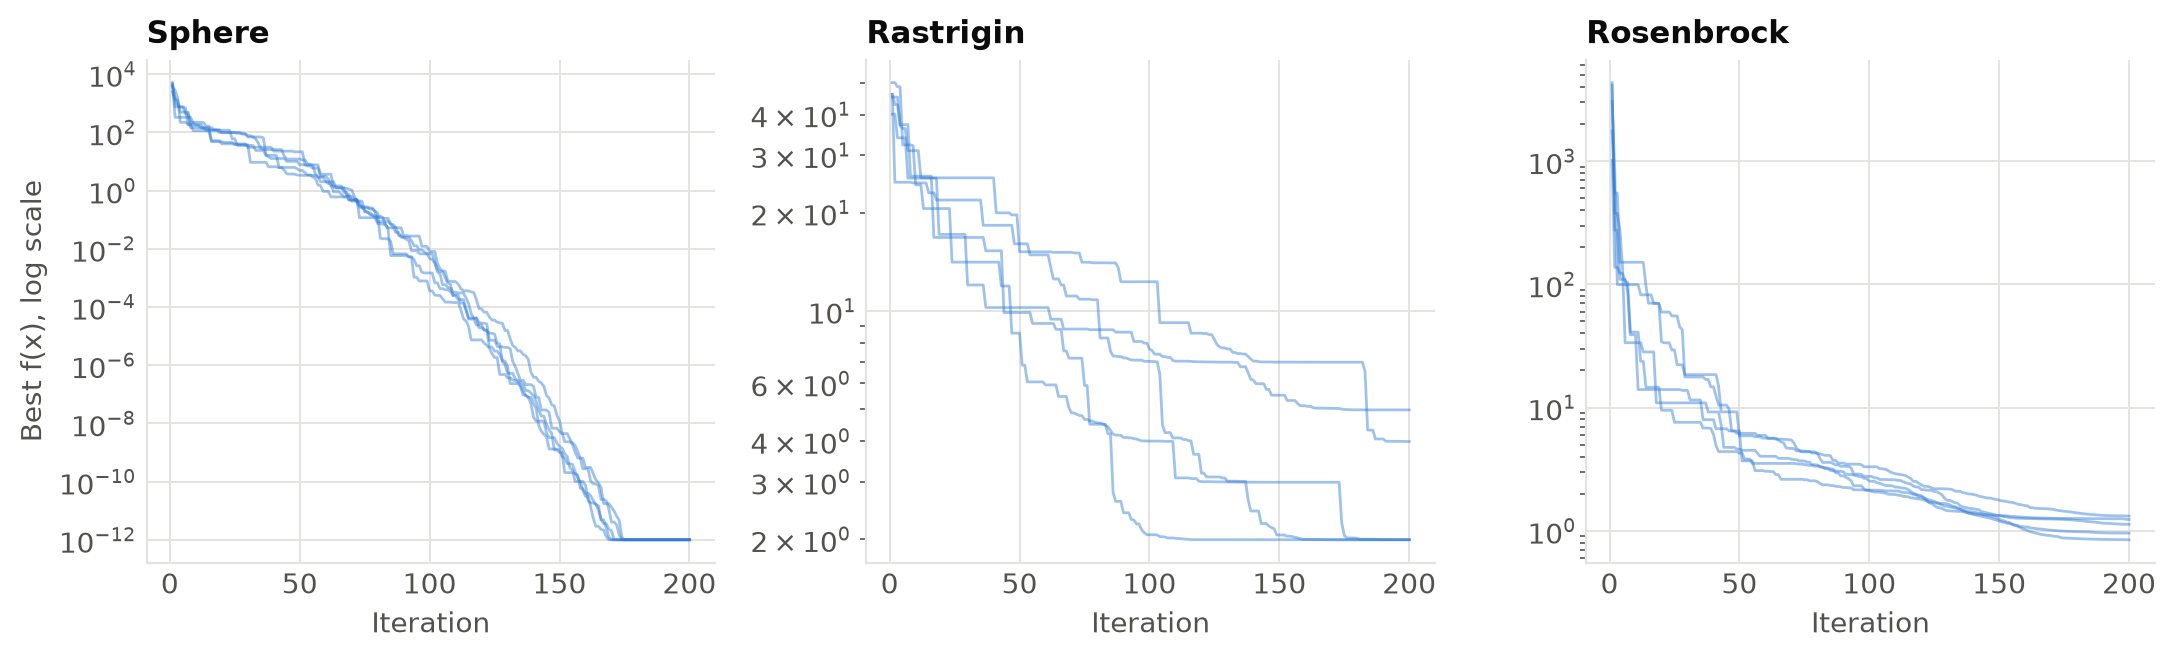
\includegraphics[width=\textwidth]{figures/16_benchmark_convergence.png}
\caption{PSO convergence on the three benchmark functions (5 runs each, log scale)}
\end{figure}

\subsection{Cross-Validation Strategy}

\topic{Time Series Cross-Validation}
For PSO fitness evaluation, walk-forward validation with an expanding window is used:
\begin{itemize}
\item 5 temporal folds over the training period
\item Each fold trains on all earlier days and validates on the next block of 519 days
\item The first fold trains on 520 days; the last trains on 2,596 days
\item Fitness = average RMSE across the 5 folds
\end{itemize}
Shuffled $k$-fold cross-validation was not used, because it would let the model train on days after the ones it is validated on.

\topic{Hold-Out Test}
The test period (2024 to 2026) is never used during the search. It is used once, to evaluate the final selected model.

\subsection{Sensitivity Analysis}

\topic{PSO Parameter Sensitivity}
The effect of PSO's own parameters was tested on the 6-dimensional Rastrigin function, with 100 iterations and 10 seeds per variant:

\begin{table}[H]
\centering
\caption{PSO parameter sensitivity on Rastrigin (lower is better)}
\begin{tabular}{|l|c|c|c|}
\hline
\textbf{Variant} & \textbf{Mean best} & \textbf{Std Dev} & \textbf{Best run} \\ \hline
Base: 20 particles, $w$ 0.9$\to$0.4, $c_1 = c_2 = 1.5$ & 6.63 & 2.61 & 2.99 \\
10 particles & 5.40 & 2.78 & 1.04 \\
40 particles & 3.59 & 2.11 & 1.00 \\
Constant inertia $w = 0.7$ & 3.73 & 1.84 & 1.99 \\
Constant inertia $w = 0.4$ & 5.27 & 2.57 & 1.00 \\
$c_1 = 2.0$, $c_2 = 1.0$ (more cognitive) & 4.77 & 3.42 & 1.00 \\
$c_1 = 1.0$, $c_2 = 2.0$ (more social) & 3.76 & 2.39 & 1.03 \\ \hline
\end{tabular}
\end{table}

Results show high run-to-run variance on this multi-modal function: standard deviations are 2 to 3 points, so differences of 1 to 2 points between variants are within noise. A larger swarm (40 particles) gave the lowest mean, as expected from its broader exploration. With only 100 iterations, the decreasing-inertia schedule spends much of the run exploring and did not beat constant $w = 0.7$; with the 25-iteration budget of the main experiment, the choice of schedule matters less than the swarm's ability to locate the right region.

\subsection{Statistical Significance Testing}

\topic{Block Bootstrap}
Daily forecast errors are autocorrelated, so ordinary resampling would overstate confidence. A moving-block bootstrap \cite{kunsch1989} resamples whole weeks (block length 7, 5,000 resamples) and computes the RMSE gain:
\begin{equation}
\Delta = RMSE_{baseline} - RMSE_{tuned}
\end{equation}
The 2.5th and 97.5th percentiles of $\Delta$ give a 95\% confidence interval.

\topic{Paired t-test}
Compares the daily squared errors of the default and tuned models:
\begin{equation}
t = \frac{\bar{d}}{s_d / \sqrt{n}}
\end{equation}
where $\bar{d}$ is the mean difference and $s_d$ the standard deviation of differences.

\topic{Wilcoxon Signed-Rank Test}
A non-parametric alternative for non-normal differences:
\begin{equation}
W = \sum_{i=1}^{n} \operatorname{sgn}(x_{2,i} - x_{1,i}) \cdot R_i
\end{equation}

\subsection{Computational Efficiency Metrics}

\topic{Training Time Analysis}
Measured for each approach:
\begin{itemize}
\item Wall-clock time per search run
\item Number of fitness evaluations, and how many were unique after caching
\item Iteration at which the global best stopped improving
\end{itemize}
The 20 search runs (PSO and random search, each with and without feature selection, 5 seeds each) were executed in parallel on 15 CPU cores.

%================================================================ 0.7
\section{Results and Discussion}

\subsection{PSO Convergence Analysis}

\topic{Fitness Evolution}
Figure 3 shows the global-best validation RMSE across iterations for all five PSO runs of the joint (hyperparameter and feature) search:
\begin{itemize}
\item Iteration 1: mean global best = 41.22 (already below the default forest's 41.52)
\item Iteration 10: mean global best = 40.20
\item Iteration 25: mean global best = 39.94; best run = 39.73
\end{itemize}
The joint search keeps improving for longer than a hyperparameter-only search, because there are many more feature subsets to explore. The global best was still improving at iterations 22 to 25 in every run, so a larger budget would probably lower the validation error further.

\begin{figure}[H]
\centering
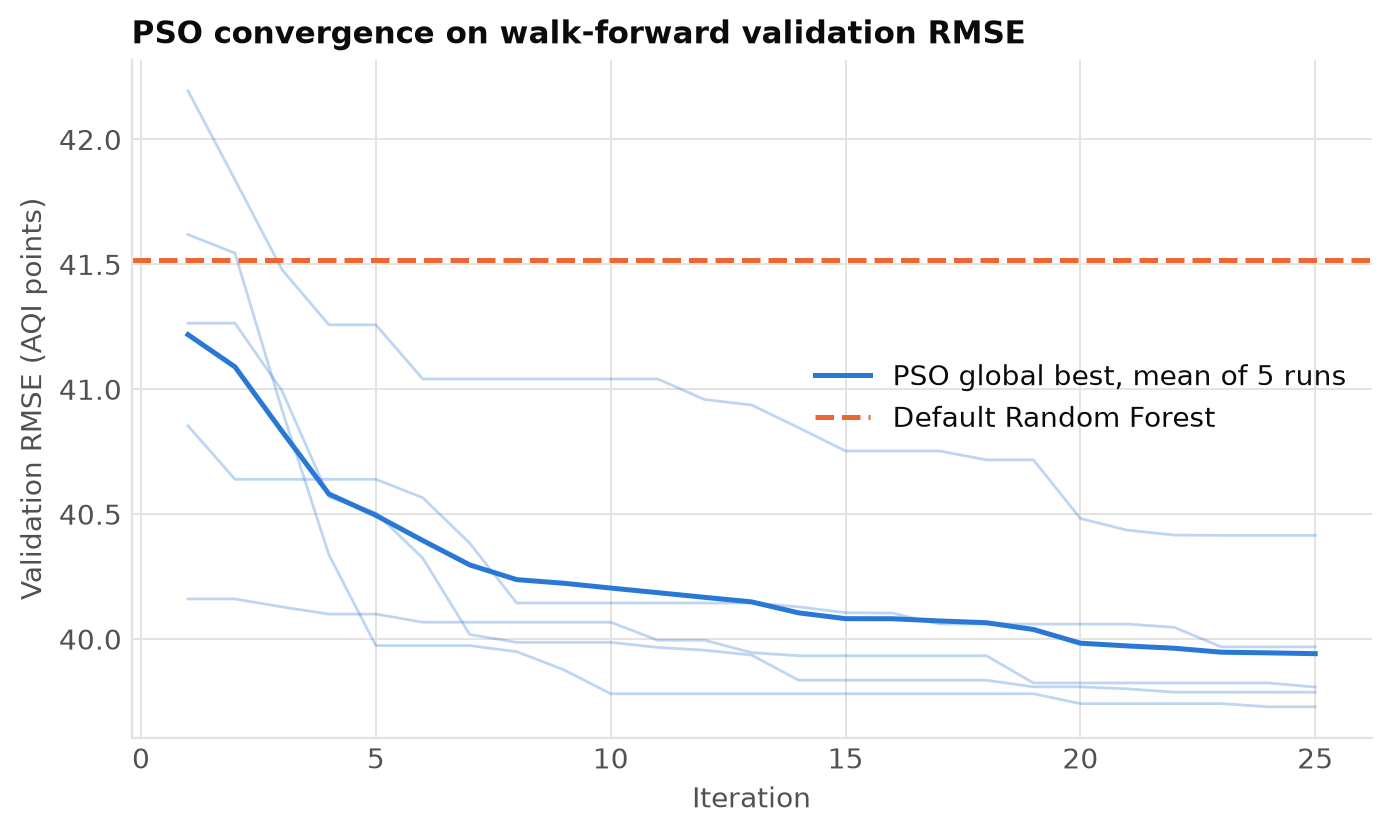
\includegraphics[width=0.88\textwidth]{figures/04_pso_convergence.png}
\caption{PSO convergence on walk-forward validation RMSE (5 runs)}
\end{figure}

\topic{Swarm Diversity}
Diversity is measured as the mean distance of particles from the swarm centre:
\begin{equation}
D_k = \frac{1}{N}\sum_{i=1}^{N}\left\lVert \mathbf{x}_i^k - \bar{\mathbf{x}}^k \right\rVert
\end{equation}
In the selected run, diversity fell from 1.28 to 0.19 while the swarm's mean RMSE fell from 42.97 to 39.85, showing the expected shift from exploration to exploitation as the inertia weight decreased. Diversity is larger than in a 6-dimensional search simply because distances are measured in 38 dimensions.

\begin{figure}[H]
\centering
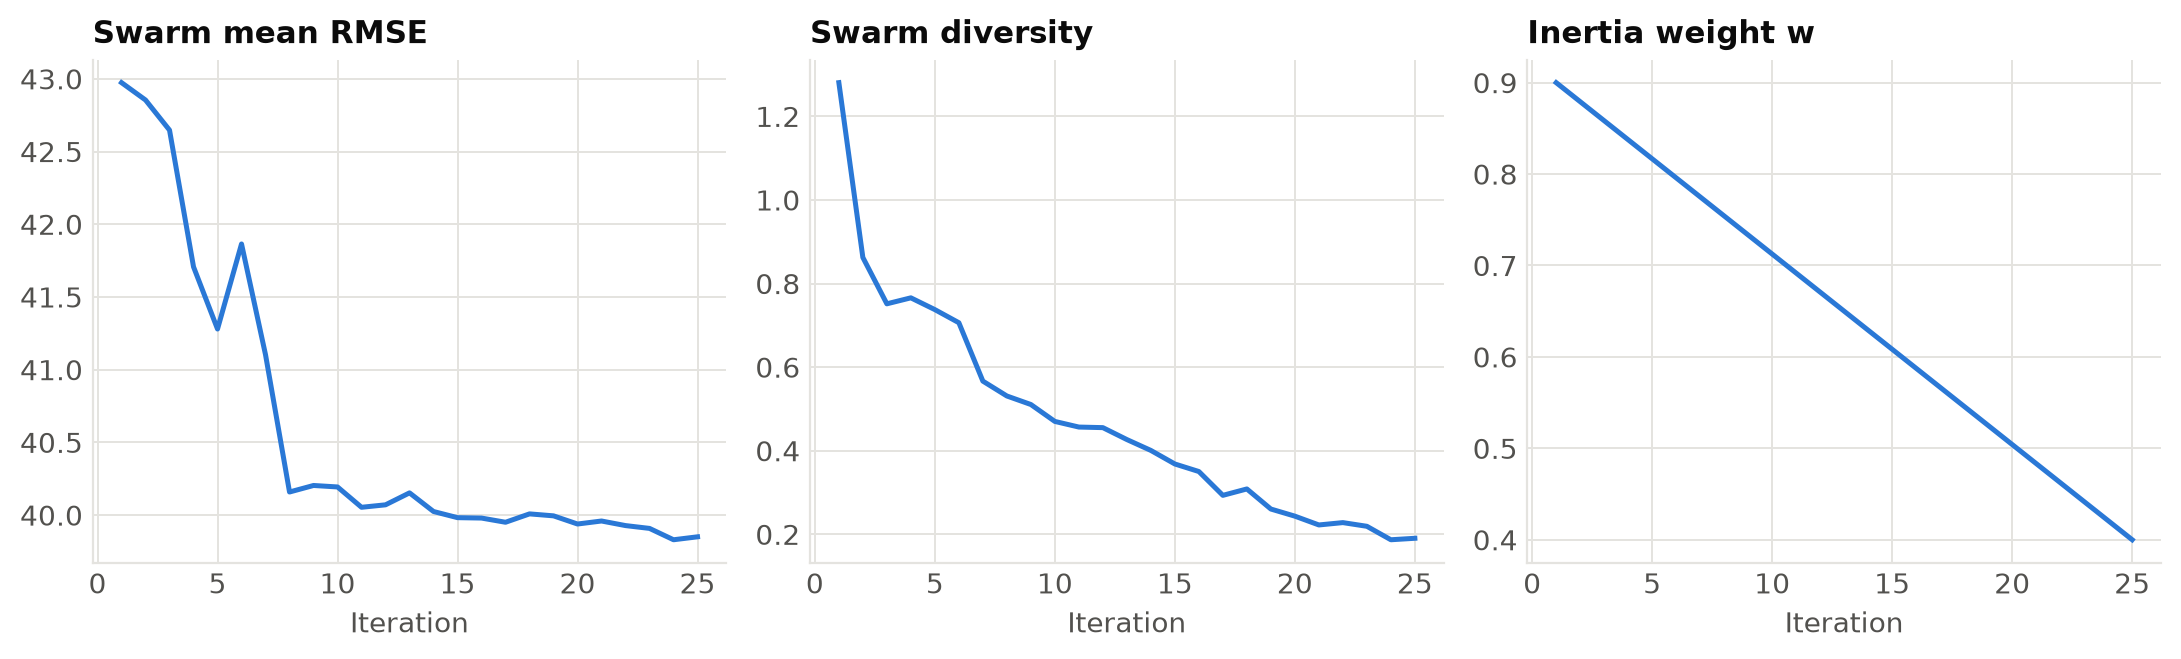
\includegraphics[width=\textwidth]{figures/06_swarm_dynamics.png}
\caption{Swarm mean fitness, diversity and inertia weight in the selected run}
\end{figure}

\subsection{Optimal Configuration}
The run with the lowest validation RMSE (seed 0, RMSE 39.73) was selected.

\begin{table}[H]
\centering
\caption{Best configuration found by PSO}
\begin{tabular}{|l|c|c|c|}
\hline
\textbf{Setting} & \textbf{Default} & \textbf{PSO, hyperparameters only} & \textbf{PSO, joint (final)} \\ \hline
n\_estimators & 100 & 291 & 224 \\
max\_depth & Unlimited & 17 & 18 \\
min\_samples\_split & 2 & 6 & 8 \\
min\_samples\_leaf & 1 & 3 & 2 \\
max\_features & 1.0 & 0.797 & 0.799 \\
max\_samples & 1.0 & 0.655 & 0.592 \\
Features used & 32 & 32 & 14 \\
Validation RMSE & 41.52 & 40.66 & \textbf{39.73} \\ \hline
\end{tabular}
\end{table}

\lead{Key Insights:}
\begin{itemize}
\item Both searches found very similar hyperparameters: depth near 17, about 80\% of features tried per split, and 60 to 65\% of days per tree
\item Limited depth and leaves of 2 to 3 days regularize each tree; feature and sample sub-sampling decorrelate the trees
\item Feature selection removed 18 of 32 features and lowered validation RMSE by a further 0.93 points
\end{itemize}

\begin{figure}[H]
\centering
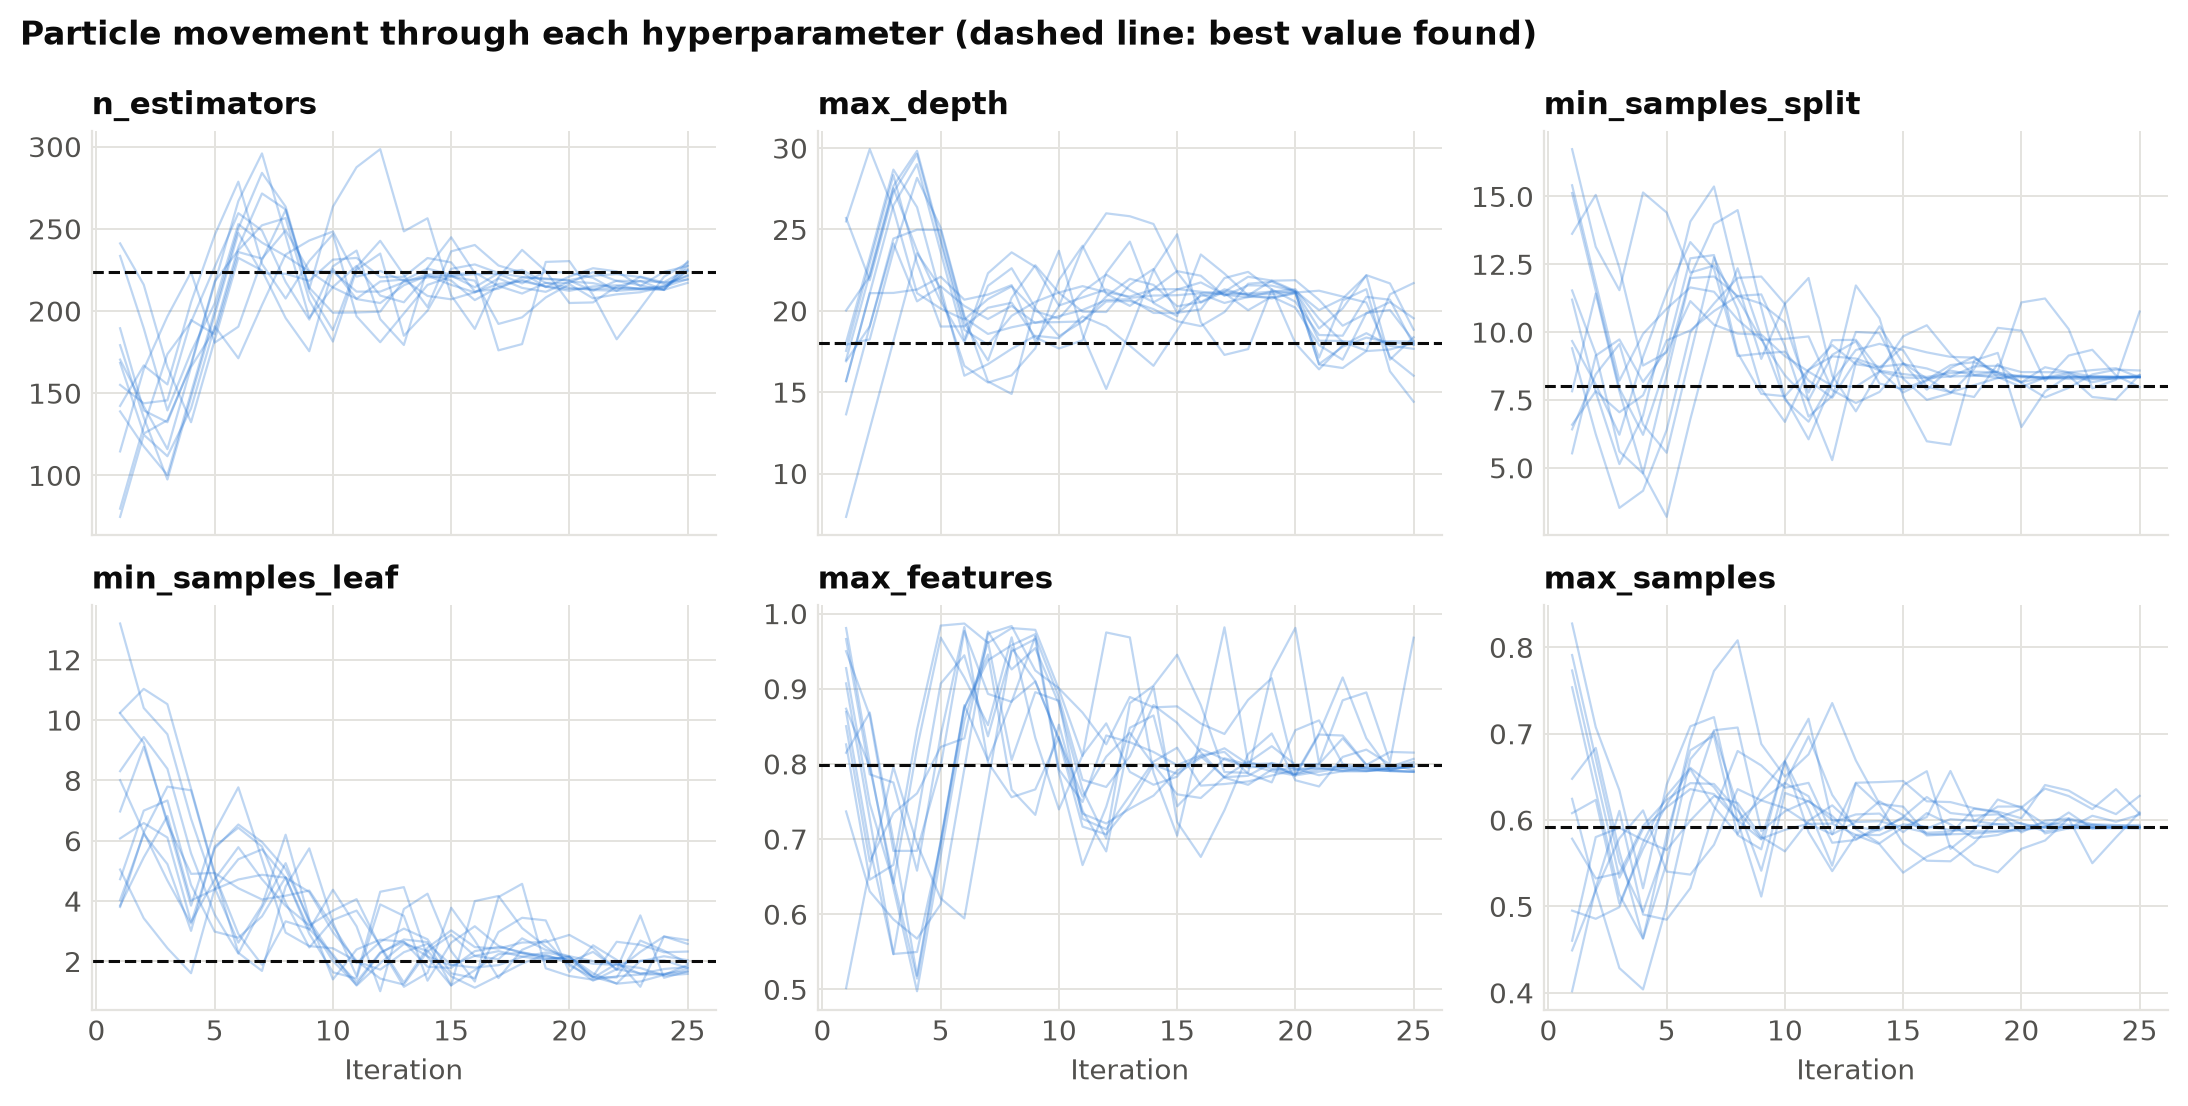
\includegraphics[width=\textwidth]{figures/07_parameter_paths.png}
\caption{Particle trajectories through each hyperparameter in the selected run}
\end{figure}

\subsection{Feature Selection Results}
The 14 features kept by the final model are: today's AQI, yesterday's AQI, the 3-day and 30-day mean AQI, the day-on-day AQI change, maximum temperature, rainfall, 3-day rainfall, maximum wind speed, the change in mean wind speed, wind direction (sine and cosine), shortwave radiation, and one day-of-week term.

\lead{Consistent choices across the five runs:}
\begin{itemize}
\item \textbf{Always kept (5 of 5 runs):} today's AQI, 3-day rainfall, shortwave radiation, wind direction (sine), change in mean wind speed, day of week (cosine)
\item \textbf{Never kept (0 of 5 runs):} relative humidity, surface pressure, dew point, and the AQI two days ago
\item The runs kept between 12 and 18 features
\end{itemize}
The kept variables are those that physically control pollution: wind and its changes disperse it, rain washes it out, and solar radiation drives the daytime mixing layer. Humidity, pressure and dew point are strongly correlated with temperature and season, so they add little once those are present. Recent AQI is represented by today's value and short averages, which makes the separate lags redundant.

\begin{figure}[H]
\centering
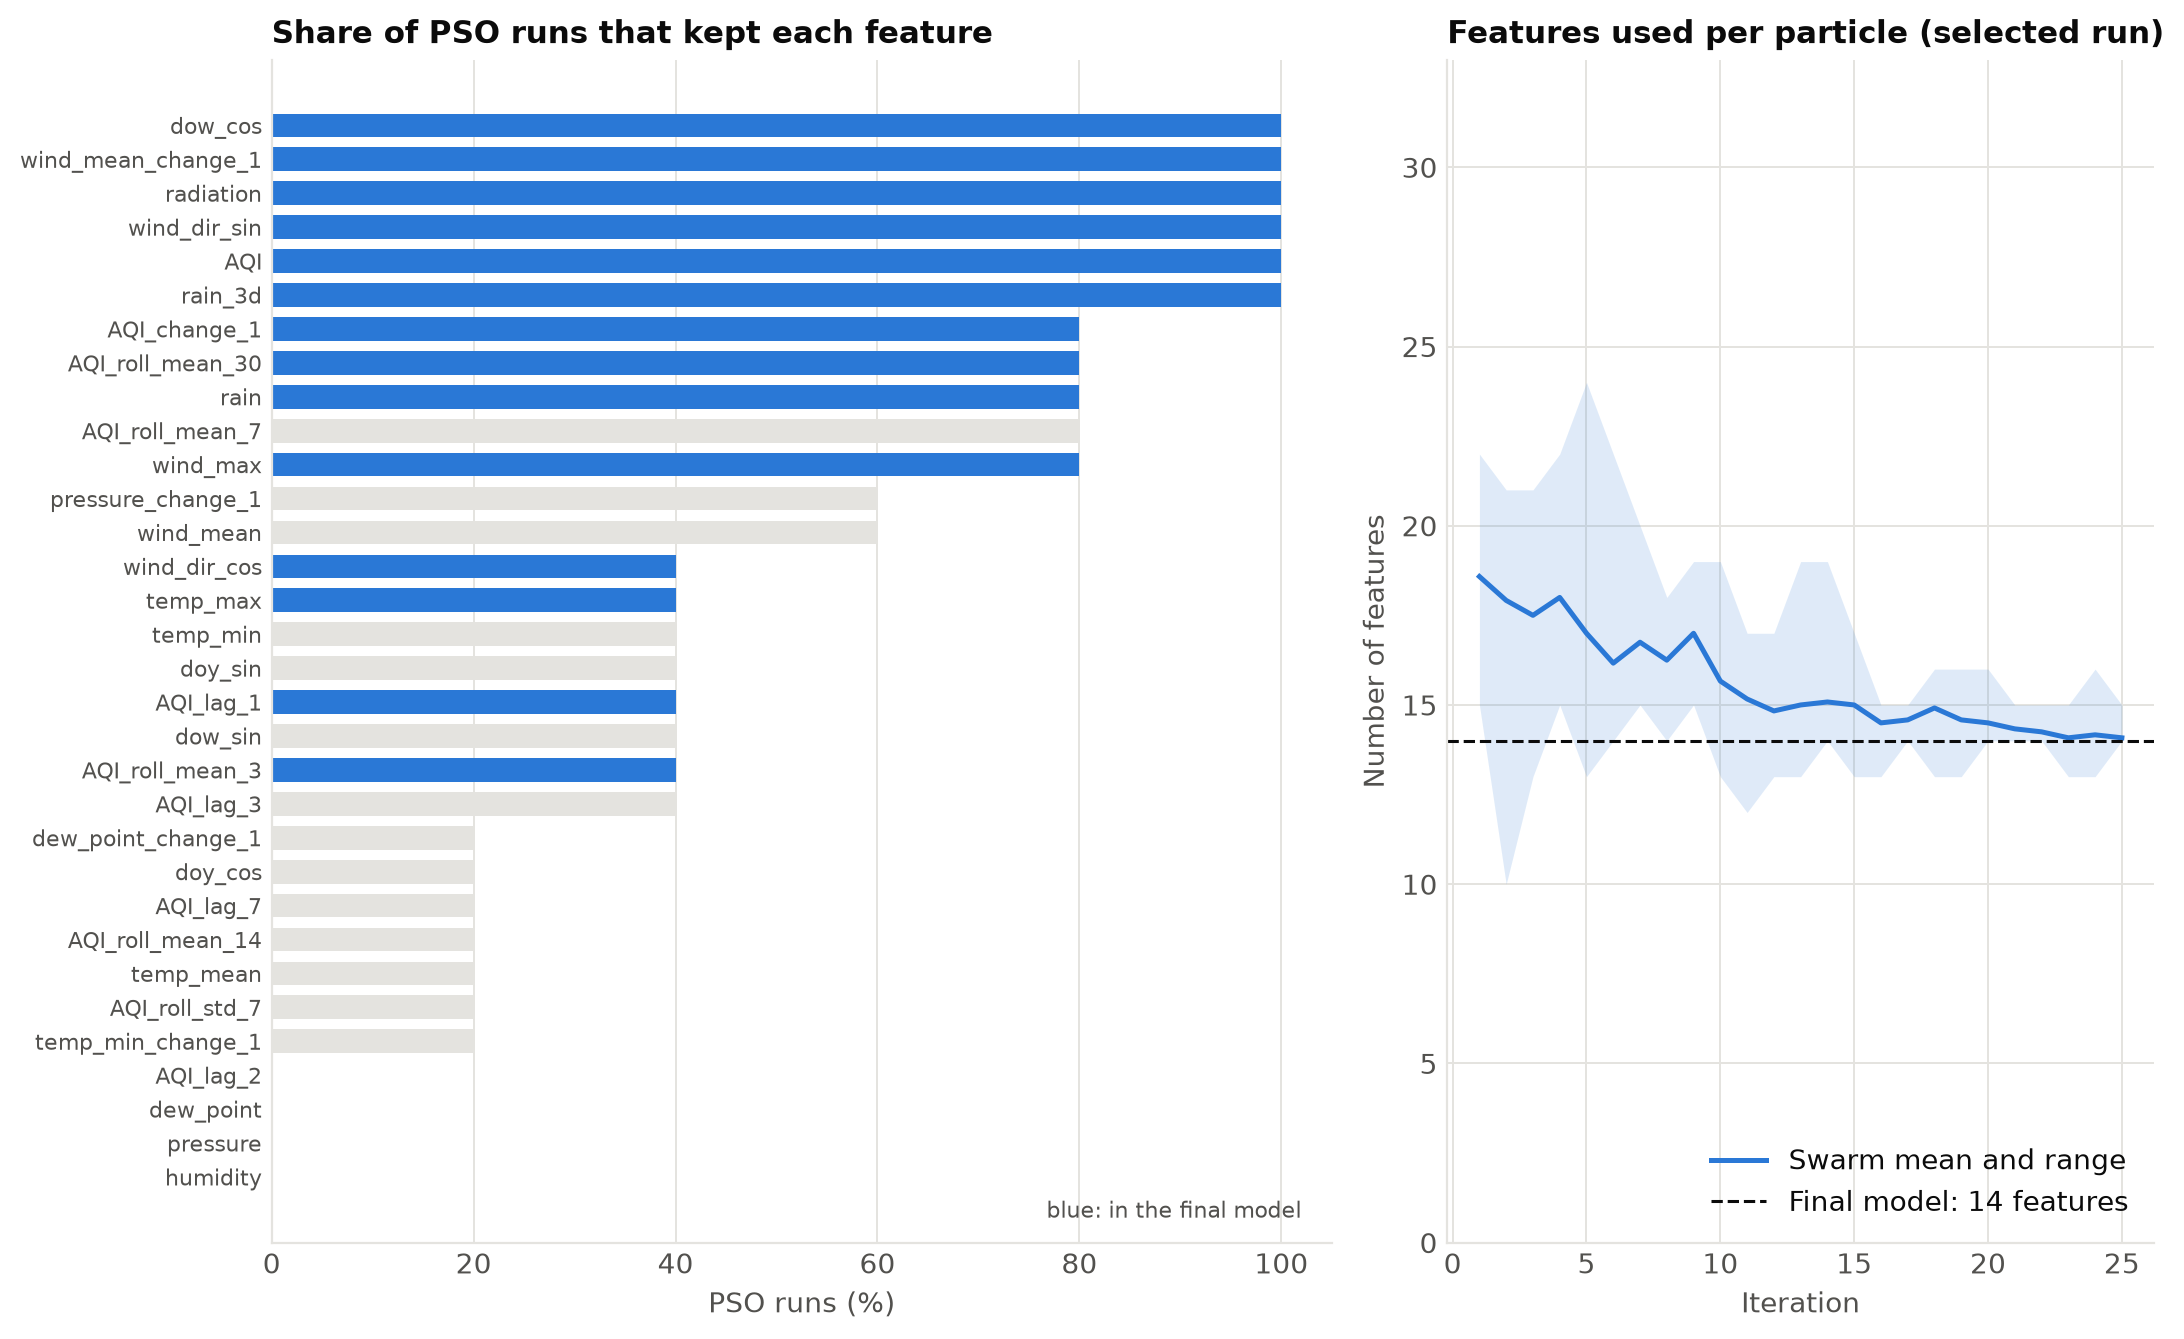
\includegraphics[width=\textwidth]{figures/17_feature_selection.png}
\caption{Share of PSO runs that kept each feature (left) and the number of features used by the swarm in the selected run (right)}
\end{figure}

\subsection{Prediction Performance}

\topic{Test Period Results}
\begin{table}[H]
\centering
\small\setlength{\tabcolsep}{4pt}
\caption{Test performance, 1 Jan 2024 -- 24 Oct 2026 (1,026 days)}
\begin{tabular}{|l|c|c|c|c|}
\hline
\textbf{Metric} & \textbf{Persistence} & \textbf{Default RF} & \textbf{PSO, hyp. only} & \textbf{PSO, joint (final)} \\ \hline
RMSE & 40.21 & 33.85 & \textbf{33.57} & 33.77 \\
MAE & 28.97 & 25.38 & \textbf{25.14} & 25.15 \\
Median absolute error & 21.00 & 19.39 & 18.87 & \textbf{18.08} \\
MAPE (\%) & 17.16 & 15.89 & 15.74 & \textbf{15.65} \\
$R^2$ & 0.832 & 0.881 & \textbf{0.883} & 0.882 \\
Category accuracy & 0.688 & \textbf{0.719} & 0.715 & 0.714 \\
Category precision (macro) & 0.547 & 0.607 & 0.611 & \textbf{0.622} \\
Category recall (macro) & 0.548 & \textbf{0.555} & 0.552 & 0.552 \\
Category F1 (macro) & 0.548 & 0.568 & 0.566 & \textbf{0.569} \\
AUC, AQI $>$ 300 & 0.978 & 0.986 & \textbf{0.987} & 0.986 \\ \hline
\end{tabular}
\end{table}

\lead{Analysis:}
\begin{itemize}
\item The final model beats the default forest on RMSE, MAE, median error, MAPE, $R^2$, category precision and F1, but by small margins (RMSE 0.25\%, median error 6.8\%)
\item It is slightly worse than the hyperparameter-only PSO model on RMSE (33.77 against 33.57), even though its validation error was much lower
\item All forests beat persistence substantially (RMSE 16.0\% lower for the final model)
\item All forests detect \emph{Very Poor} or worse days very well (AUC 0.986 to 0.987)
\end{itemize}

\begin{figure}[H]
\centering
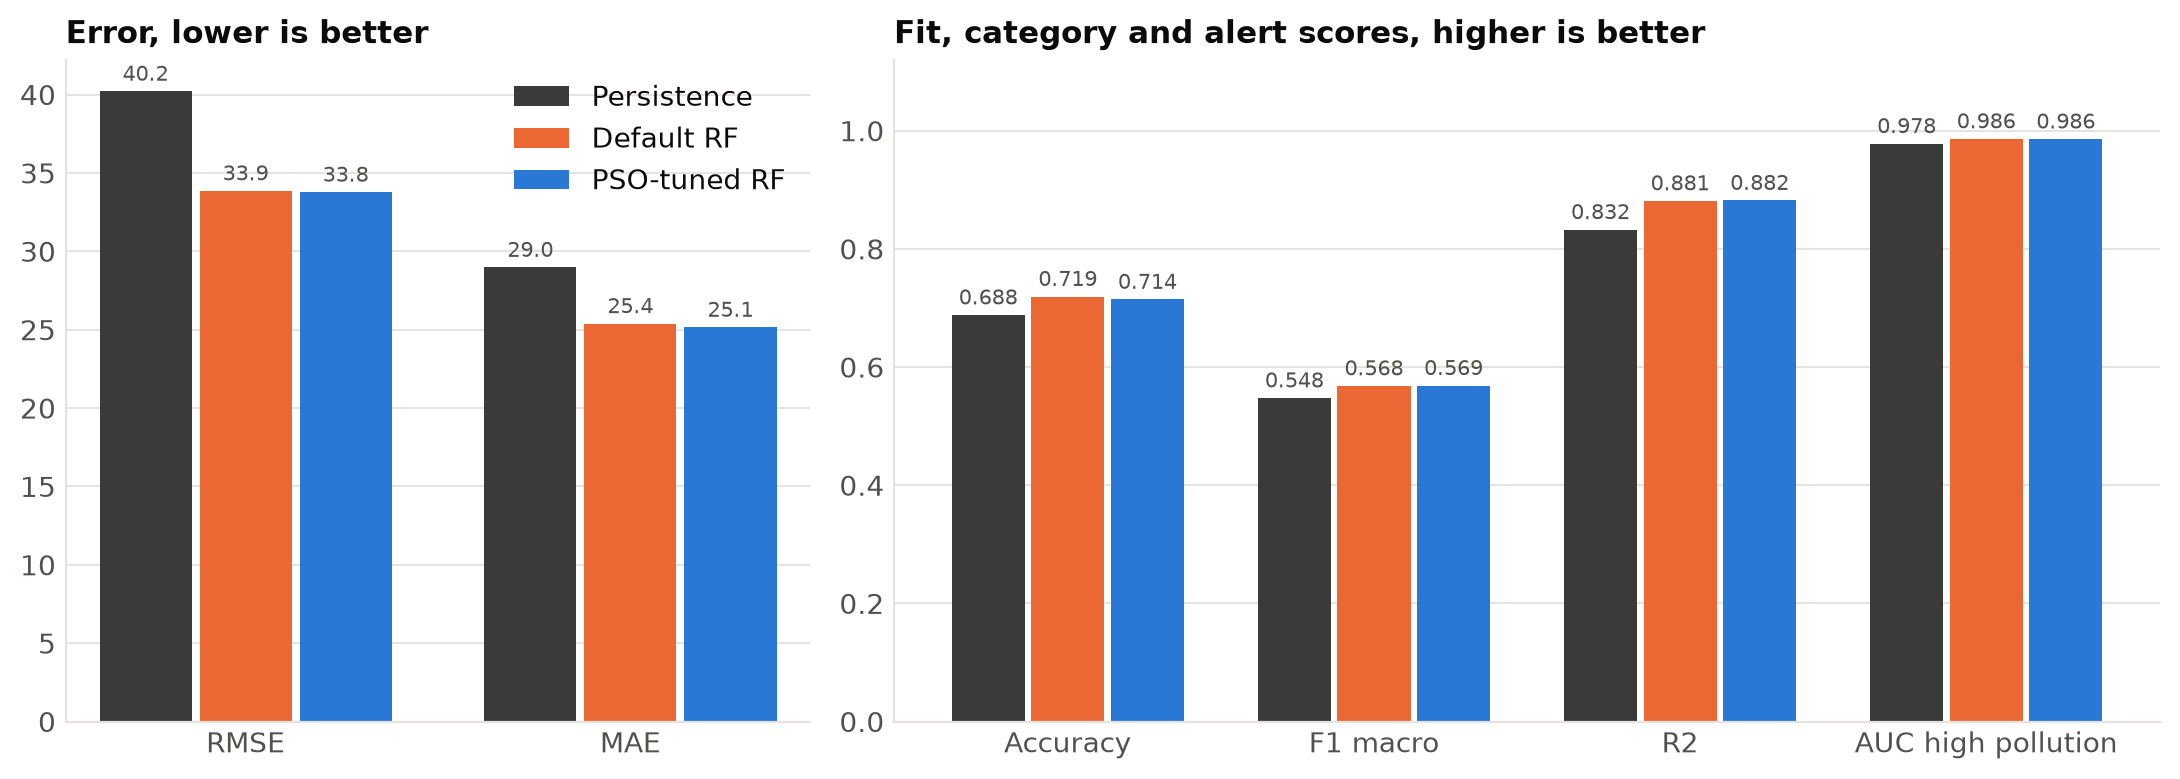
\includegraphics[width=\textwidth]{figures/08_metric_comparison.png}
\caption{Test metrics of persistence, the default forest and the final PSO model}
\end{figure}

\subsection{Temporal Performance Analysis}

\topic{Performance Across Years and Seasons}
\begin{table}[H]
\centering
\small\setlength{\tabcolsep}{4pt}
\caption{Test RMSE by period}
\begin{tabular}{|l|c|c|c|c|c|c|}
\hline
\textbf{Period} & \textbf{Days} & \textbf{Mean AQI} & \textbf{Persist.} & \textbf{Default RF} & \textbf{PSO hyp.} & \textbf{PSO joint} \\ \hline
2024 & 365 & 208.6 & 41.98 & \textbf{34.12} & 34.20 & 34.30 \\
2025 & 365 & 201.0 & 38.38 & 34.23 & \textbf{33.66} & 34.07 \\
2026 (to 24 Oct) & 296 & 166.6 & 40.17 & 33.04 & \textbf{32.67} & 32.72 \\
Winter (Oct--Feb) & 385 & 281.6 & 48.29 & 40.22 & \textbf{40.16} & 40.22 \\
Rest of year (Mar--Sep) & 641 & 141.0 & 34.45 & 29.37 & \textbf{28.90} & 29.21 \\ \hline
\end{tabular}
\end{table}

Errors are largest in the winter smog season, when AQI is highest and most volatile. In every period the three forests are within 0.6 points of each other, while persistence is 4 to 8 points worse.

\begin{figure}[H]
\centering
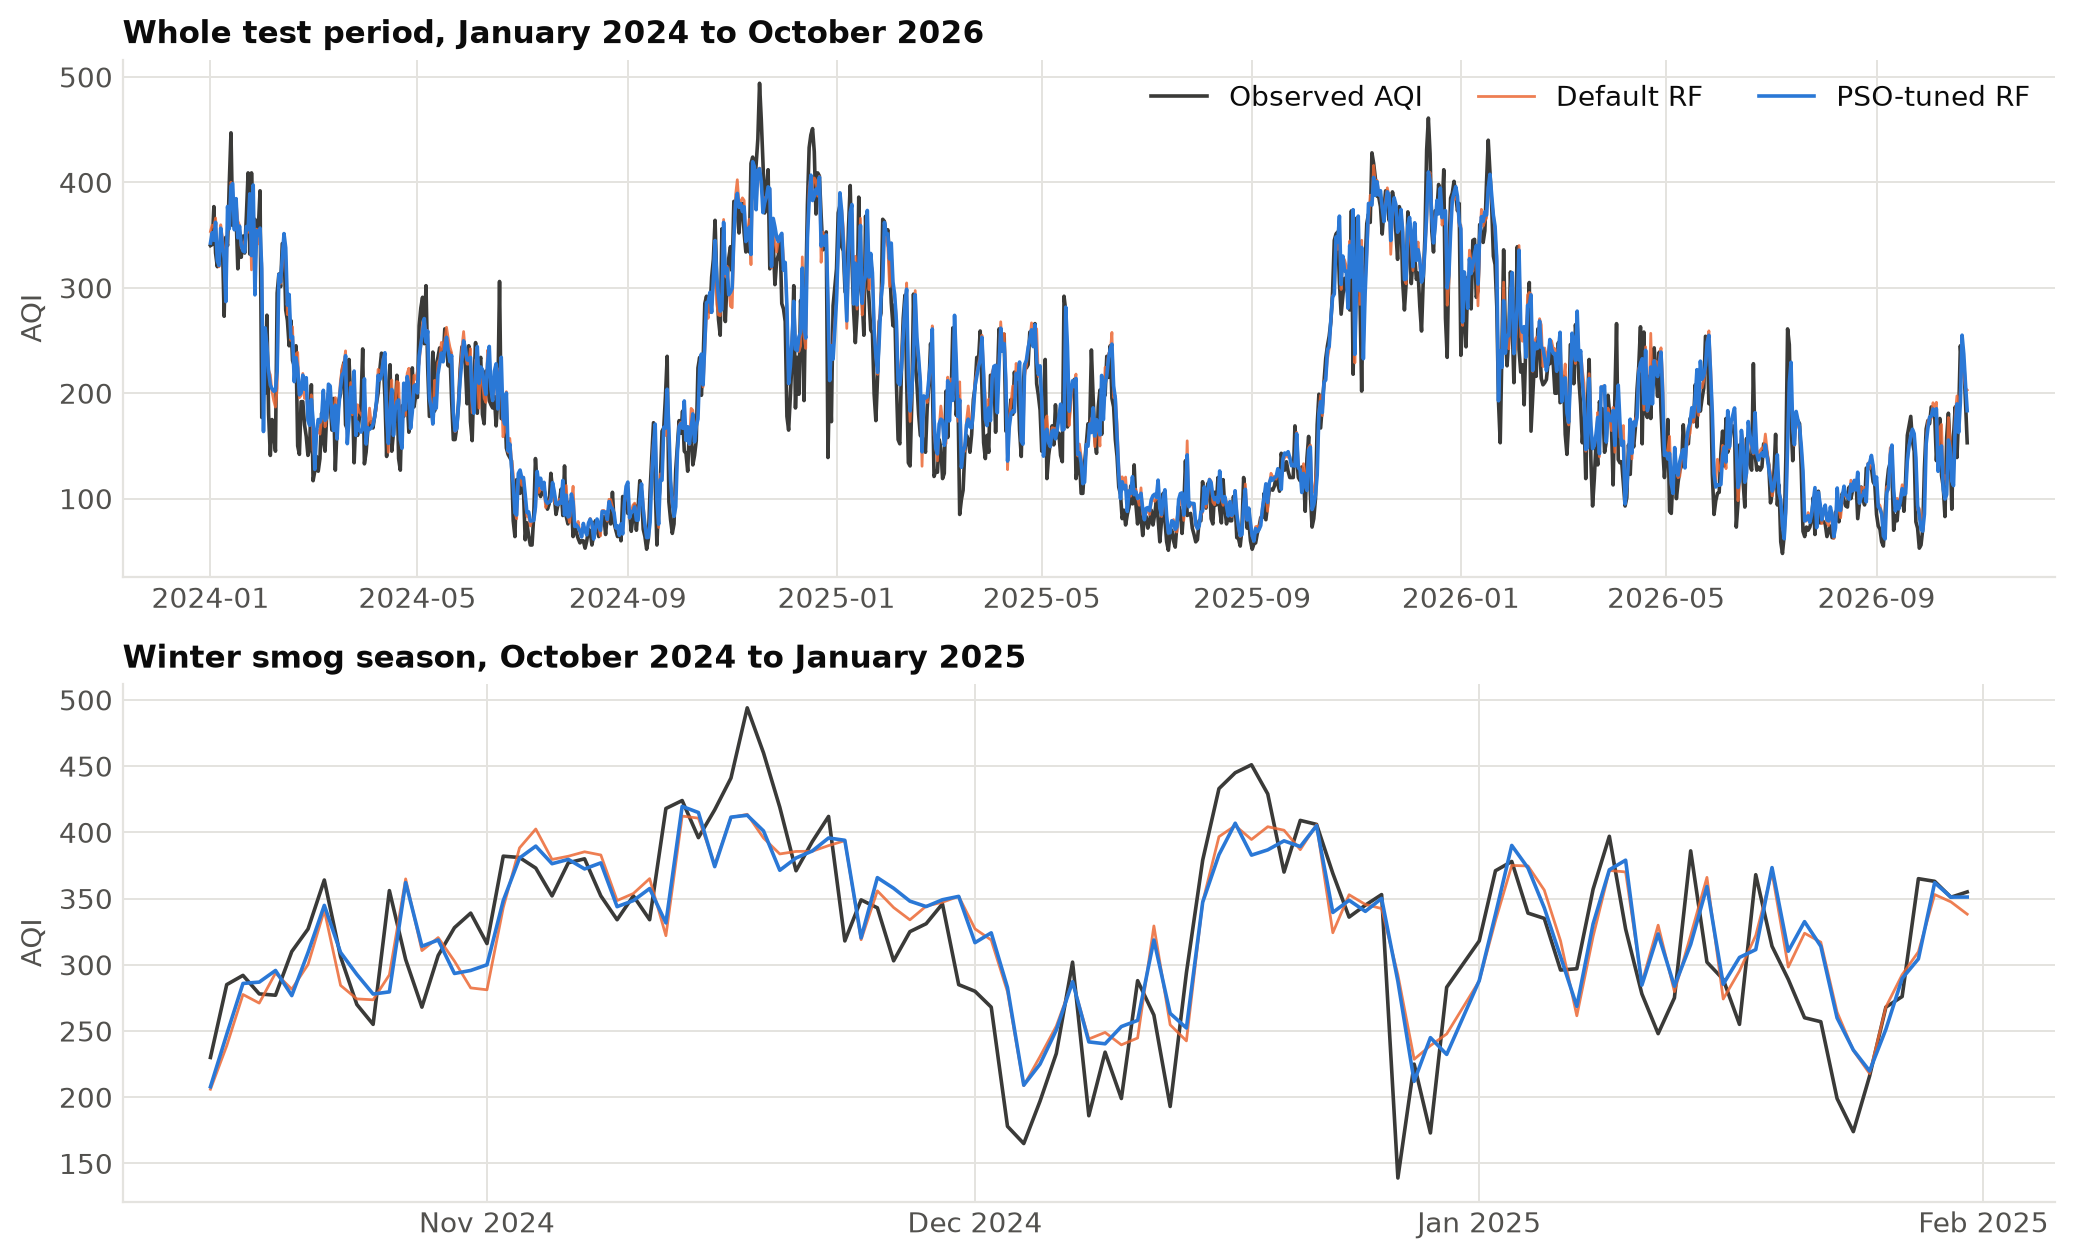
\includegraphics[width=\textwidth]{figures/09_forecast_timeline.png}
\caption{Observed and forecast AQI over the test period, with the 2024--25 winter in detail}
\end{figure}

\subsection{Comparison with Baseline Models}

\topic{Performance Comparison}
\begin{table}[H]
\centering
\caption{Model comparison on the test period}
\begin{tabular}{|l|c|c|c|}
\hline
\textbf{Model} & \textbf{RMSE} & \textbf{MAE} & \textbf{$R^2$} \\ \hline
Persistence & 40.21 & 28.97 & 0.832 \\
Default Random Forest & 33.85 & 25.38 & 0.881 \\
\textbf{PSO Random Forest, joint (final)} & \textbf{33.77} & \textbf{25.15} & \textbf{0.882} \\
Gradient Boosting (default) & 33.61 & 25.33 & 0.883 \\
PSO Random Forest, hyperparameters only & 33.57 & 25.14 & 0.883 \\
Support Vector Regression & 33.46 & 25.40 & 0.884 \\
Ridge regression & 33.45 & 25.27 & 0.884 \\ \hline
\end{tabular}
\end{table}

\lead{Key Findings:}
\begin{itemize}
\item All learned models fall within 0.4 RMSE points of each other and beat persistence by 16 to 17\%
\item Ridge regression and SVR have the lowest RMSE. With good lag and weather features, next-day AQI is close to a linear problem
\item The final PSO model uses less than half the features of every other model at very similar accuracy
\end{itemize}

\begin{figure}[H]
\centering
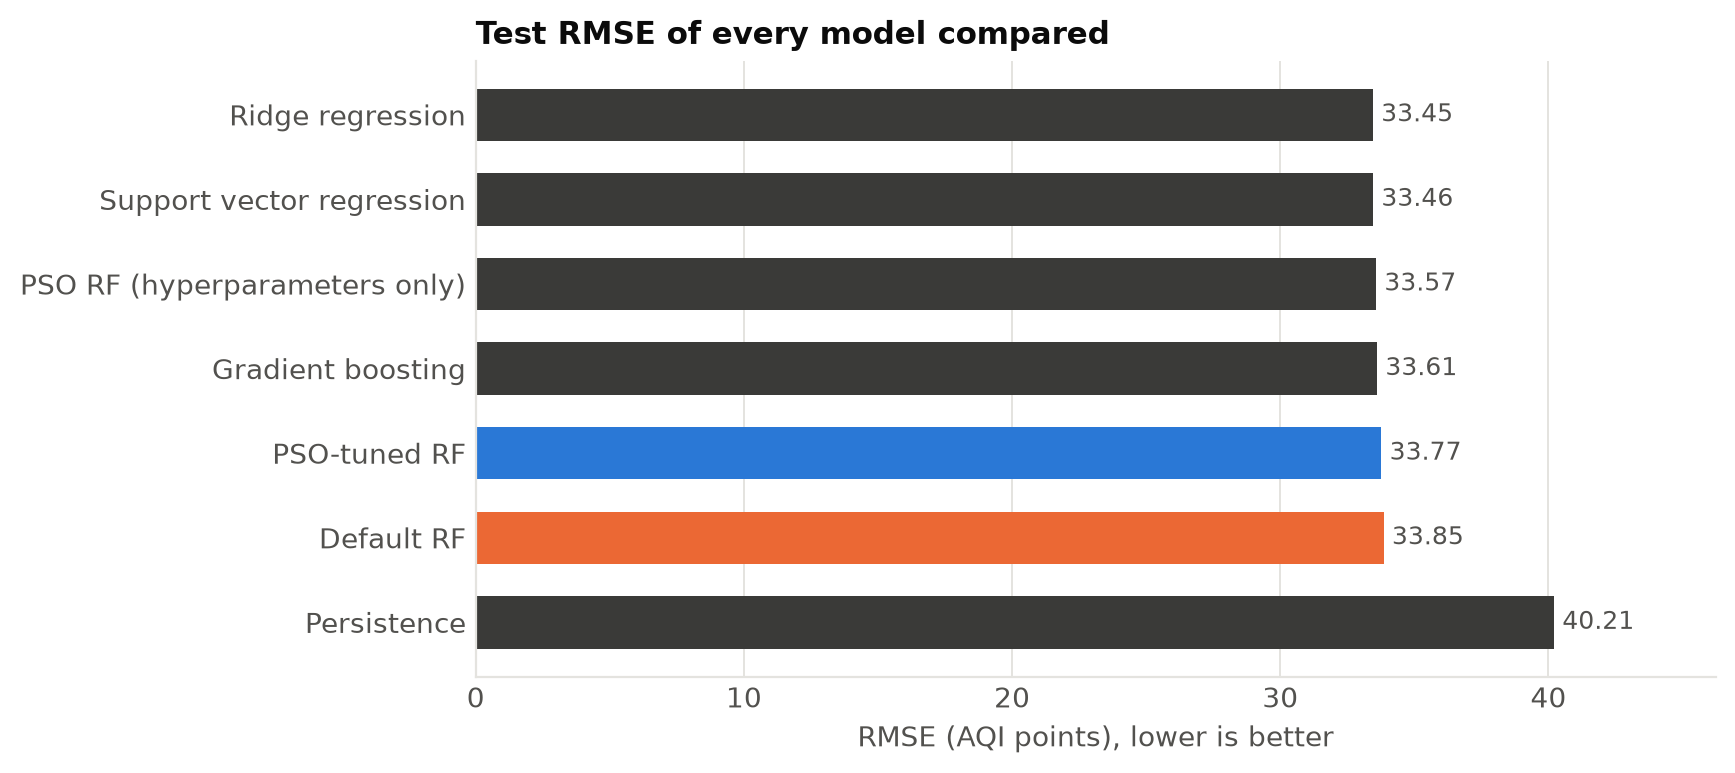
\includegraphics[width=0.82\textwidth]{figures/15_model_comparison.png}
\caption{Test RMSE of every model}
\end{figure}

\topic{PSO versus Random Search}
\begin{table}[H]
\centering
\small\setlength{\tabcolsep}{4pt}
\caption{PSO and random search with the same 312-evaluation budget (RMSE, 5 runs each)}
\begin{tabular}{|l|c|c|c|}
\hline
\textbf{Method} & \textbf{Best val.} & \textbf{Mean val.} & \textbf{Mean test} \\ \hline
Default RF & 41.52 & 41.52 & 33.81 \\
Random search, hyperparameters only & 40.75 & 40.82 & 33.62 \\
PSO, hyperparameters only & 40.66 & 40.70 & 33.55 \\
Random search, joint & 40.04 & 40.54 & 33.96 \\
\textbf{PSO, joint} & \textbf{39.73} & \textbf{39.94} & \textbf{33.47} \\ \hline
\end{tabular}
\end{table}
Test RMSE is averaged over 10 forest seeds and over the five runs of each method. In both search spaces PSO beat random search on mean validation and mean test error. The advantage is larger in the 38-dimensional joint space (0.60 validation points) than in the 6-dimensional space (0.12), because unguided sampling becomes much less effective as the number of dimensions grows. Four of the five joint PSO runs beat the best joint random-search run. Over its five runs, joint PSO also has the lowest mean test RMSE of any search (33.47, 1.0\% below the default forest).

\begin{figure}[H]
\centering
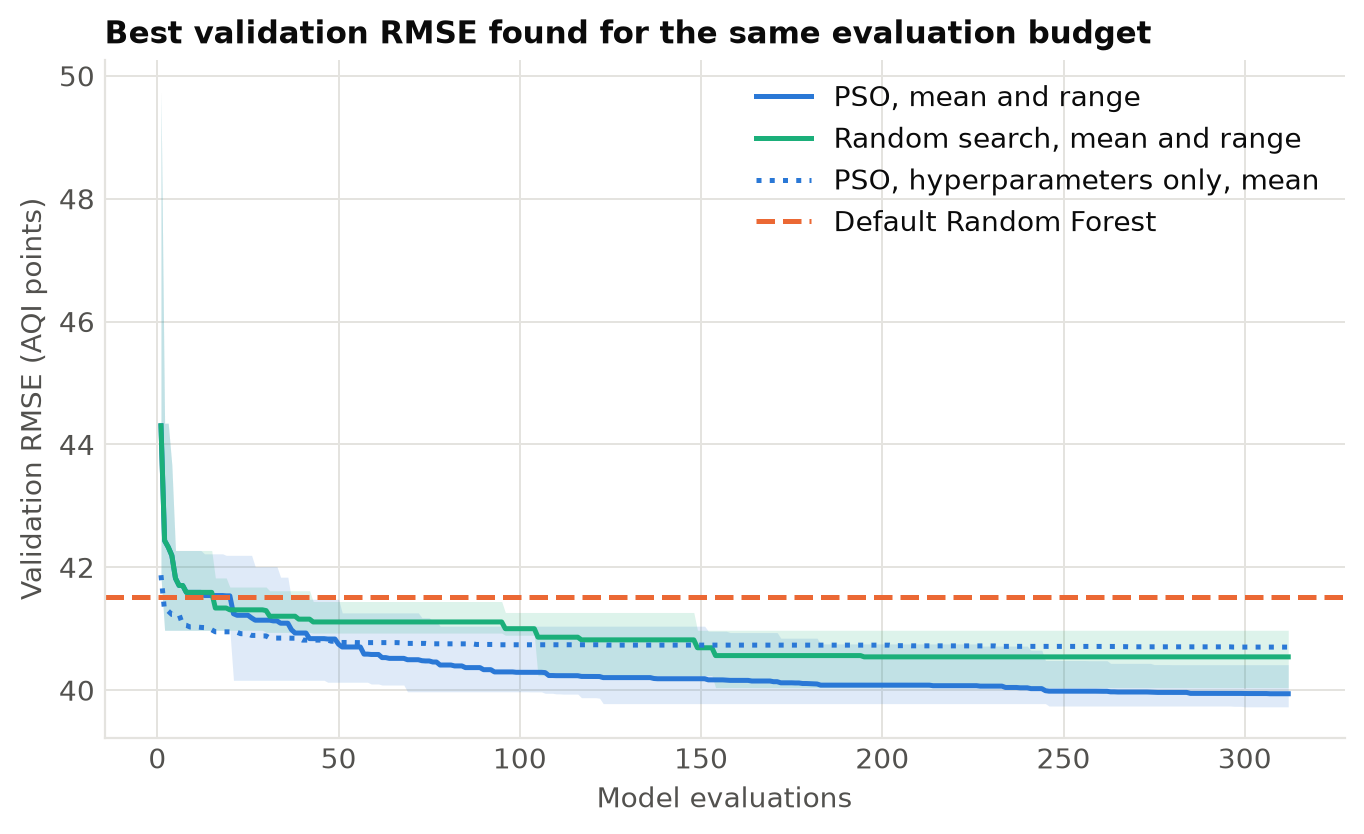
\includegraphics[width=0.88\textwidth]{figures/05_pso_vs_random_search.png}
\caption{Best validation RMSE found by PSO and random search for the same evaluation budget}
\end{figure}

\topic{Statistical Significance}
Comparison of the final PSO model with the default forest on the test period:
\begin{itemize}
\item Block-bootstrap RMSE gain: 0.09 AQI points, 95\% CI $-$0.41 to 0.59 (positive in 61.7\% of resamples)
\item Paired $t$-test on squared errors: $t = 0.31$, $p = 0.76$
\item Wilcoxon signed-rank test: $p = 0.66$
\item Final model more accurate on 49.9\% of days
\item Against persistence: gain 6.44 points, 95\% CI 4.85 to 8.06 ($p < 0.001$)
\item Against the hyperparameter-only PSO model: $-$0.20 points, 95\% CI $-$0.67 to 0.26 ($t$-test $p = 0.40$)
\end{itemize}
The improvement over persistence is highly significant. The differences between the default forest and the two PSO models are not statistically significant.

\subsection{Hyperparameter Importance Analysis}

\topic{Correlation with Performance}
Spearman correlation between each setting and validation RMSE, over all 1,560 unique configurations evaluated across the five joint PSO runs (negative means larger values lower the error):

\begin{table}[H]
\centering
\caption{Setting--fitness correlation}
\begin{tabular}{|l|c|}
\hline
\textbf{Setting} & \textbf{Spearman $\rho$ with RMSE} \\ \hline
min\_samples\_leaf & 0.659 \\
max\_depth & $-$0.346 \\
max\_samples & 0.344 \\
max\_features & $-$0.336 \\
n\_estimators & $-$0.304 \\
min\_samples\_split & 0.221 \\
Number of features used & $-$0.138 \\ \hline
\end{tabular}
\end{table}
Leaf size has the strongest effect: large leaves underfit, and the best runs used leaves of 2 to 5 days. More trees, deeper trees and more features per split all helped. The weak negative correlation for the number of features shows that the choice of \emph{which} features matters more than how many.

\subsection{Feature Importance Results}
\begin{table}[H]
\centering
\caption{Top 10 most important features of the final model (impurity-based)}
\begin{tabular}{|l|c|}
\hline
\textbf{Feature} & \textbf{Importance} \\ \hline
AQI today ($AQI_t$) & 0.635 \\
3-day mean AQI & 0.176 \\
AQI yesterday & 0.032 \\
Maximum wind speed & 0.029 \\
30-day mean AQI & 0.024 \\
Change in mean wind speed & 0.019 \\
Shortwave radiation & 0.017 \\
Rainfall & 0.016 \\
Wind direction (sine) & 0.014 \\
3-day rainfall & 0.009 \\ \hline
\end{tabular}
\end{table}
Today's AQI dominates, and AQI history accounts for 88\% of total importance. Wind, rain and radiation are the most useful weather variables: they control how quickly pollution disperses or is washed out.

\begin{figure}[H]
\centering
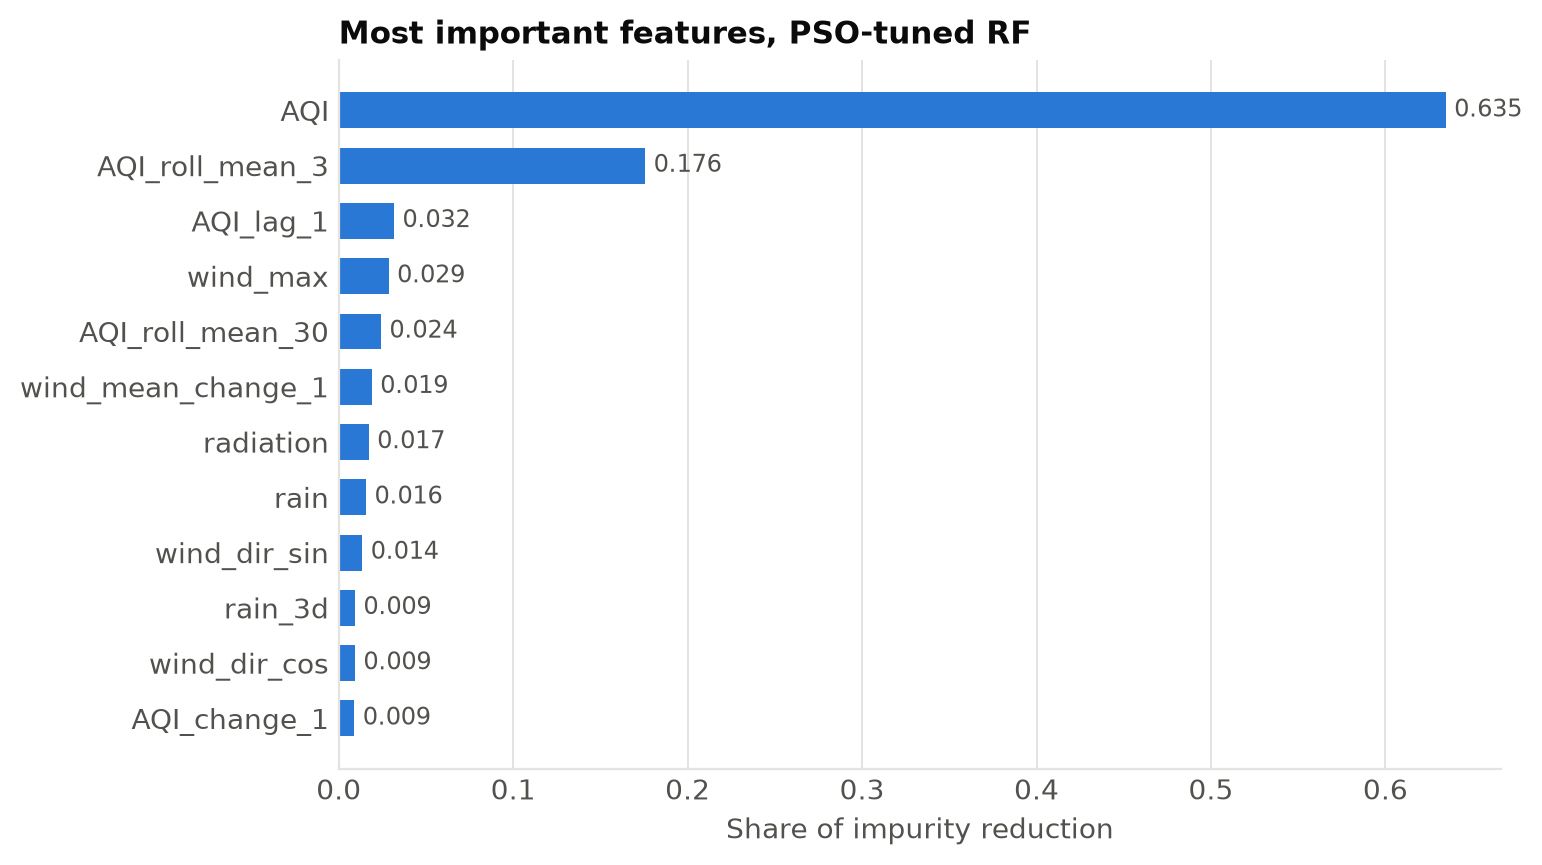
\includegraphics[width=0.75\textwidth]{figures/13_feature_importance.png}
\caption{Feature importance of the final PSO model}
\end{figure}

\subsection{Error Analysis}

\topic{Residual Distribution}
Residuals (observed minus predicted) of the final model:
\begin{itemize}
\item Mean: $-$7.72 (the model over-predicts on average)
\item Std Dev: 32.89
\item Skewness: $-$0.16 (nearly symmetric)
\item Kurtosis: 4.67 (heavier tails than a normal distribution)
\end{itemize}
Shapiro--Wilk test: $p = 1.3\times10^{-10}$, so normality is rejected because of the heavy tails.

The negative mean reflects a downward trend: the test period's mean AQI (193.8) is lower than the training period's (216.9), and the model, trained mostly on dirtier years, forecasts slightly high (mean forecast 201.5).

\begin{figure}[H]
\centering
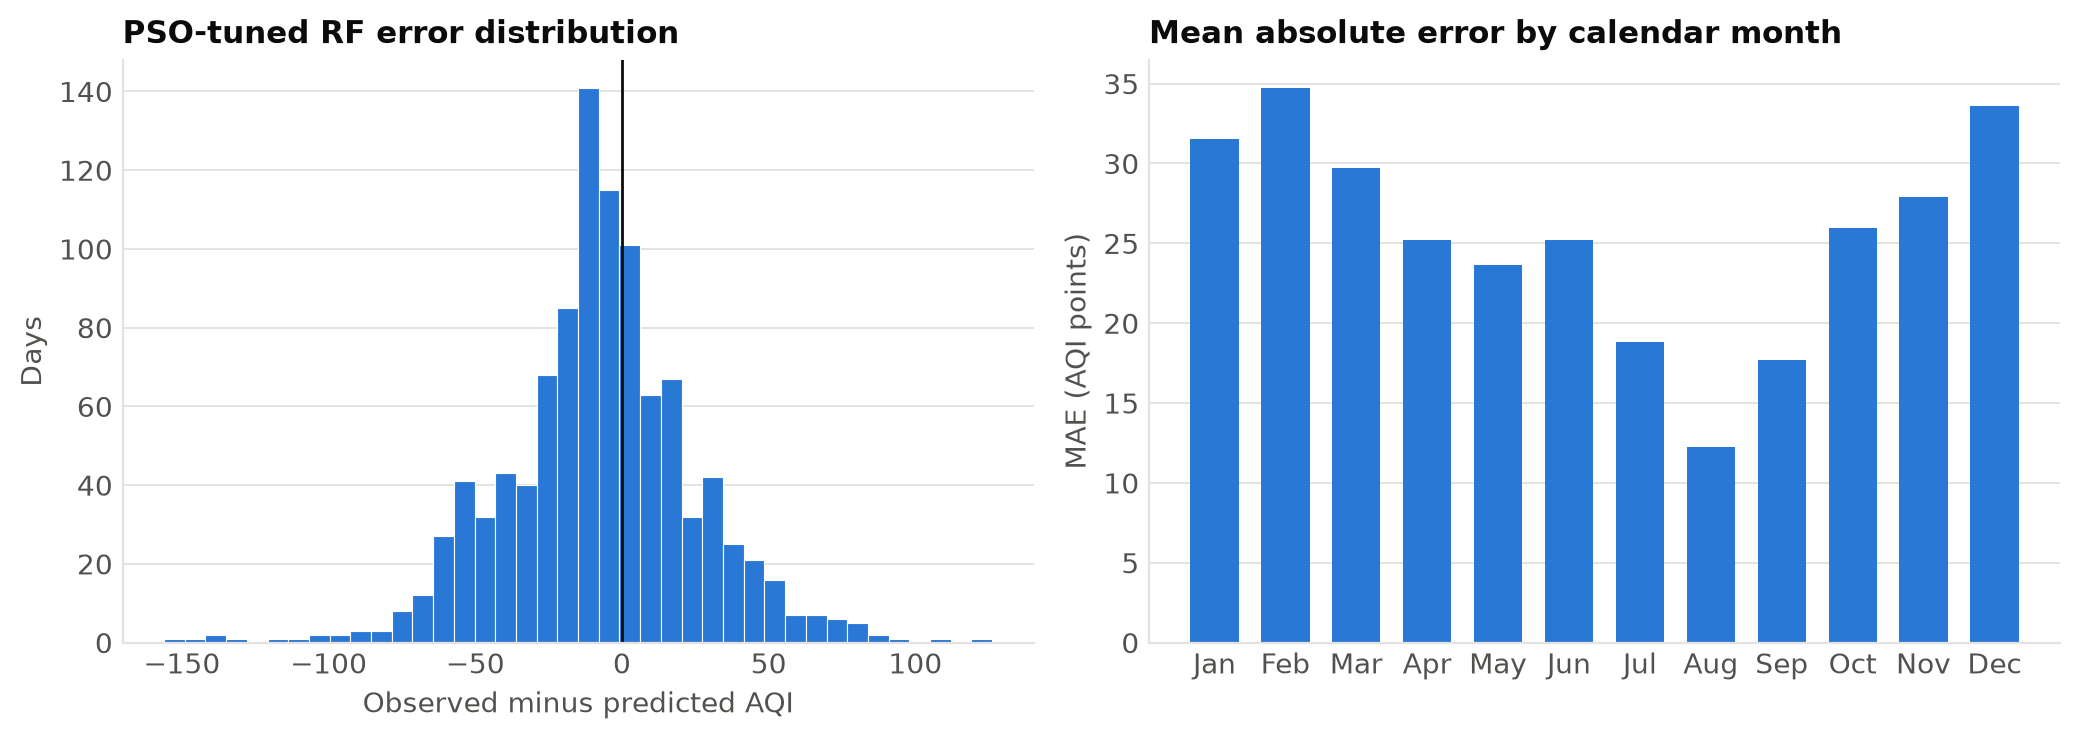
\includegraphics[width=\textwidth]{figures/11_residuals.png}
\caption{Residual distribution and mean absolute error by month}
\end{figure}

\topic{Lag on Sharp Changes}
The forecasts correlate more strongly with the previous day's AQI (0.976) than with the day being forecast (0.942), so sharp changes are followed a day late. On the 28 test days when AQI moved by more than 100 points, MAE was 87.0, against 23.4 on all other days. Such jumps are driven by events the features do not capture, such as sudden stubble-burning plumes, fireworks or a passing western disturbance.

\topic{Category Errors}
Of the 1,026 test days, 293 were placed in the wrong CPCB category, and 292 of these were only one category away. \emph{Severe} days are rare (27 days) and hard to forecast: 10 were predicted as \emph{Severe}, most of the rest as \emph{Very Poor}.

\begin{figure}[H]
\centering
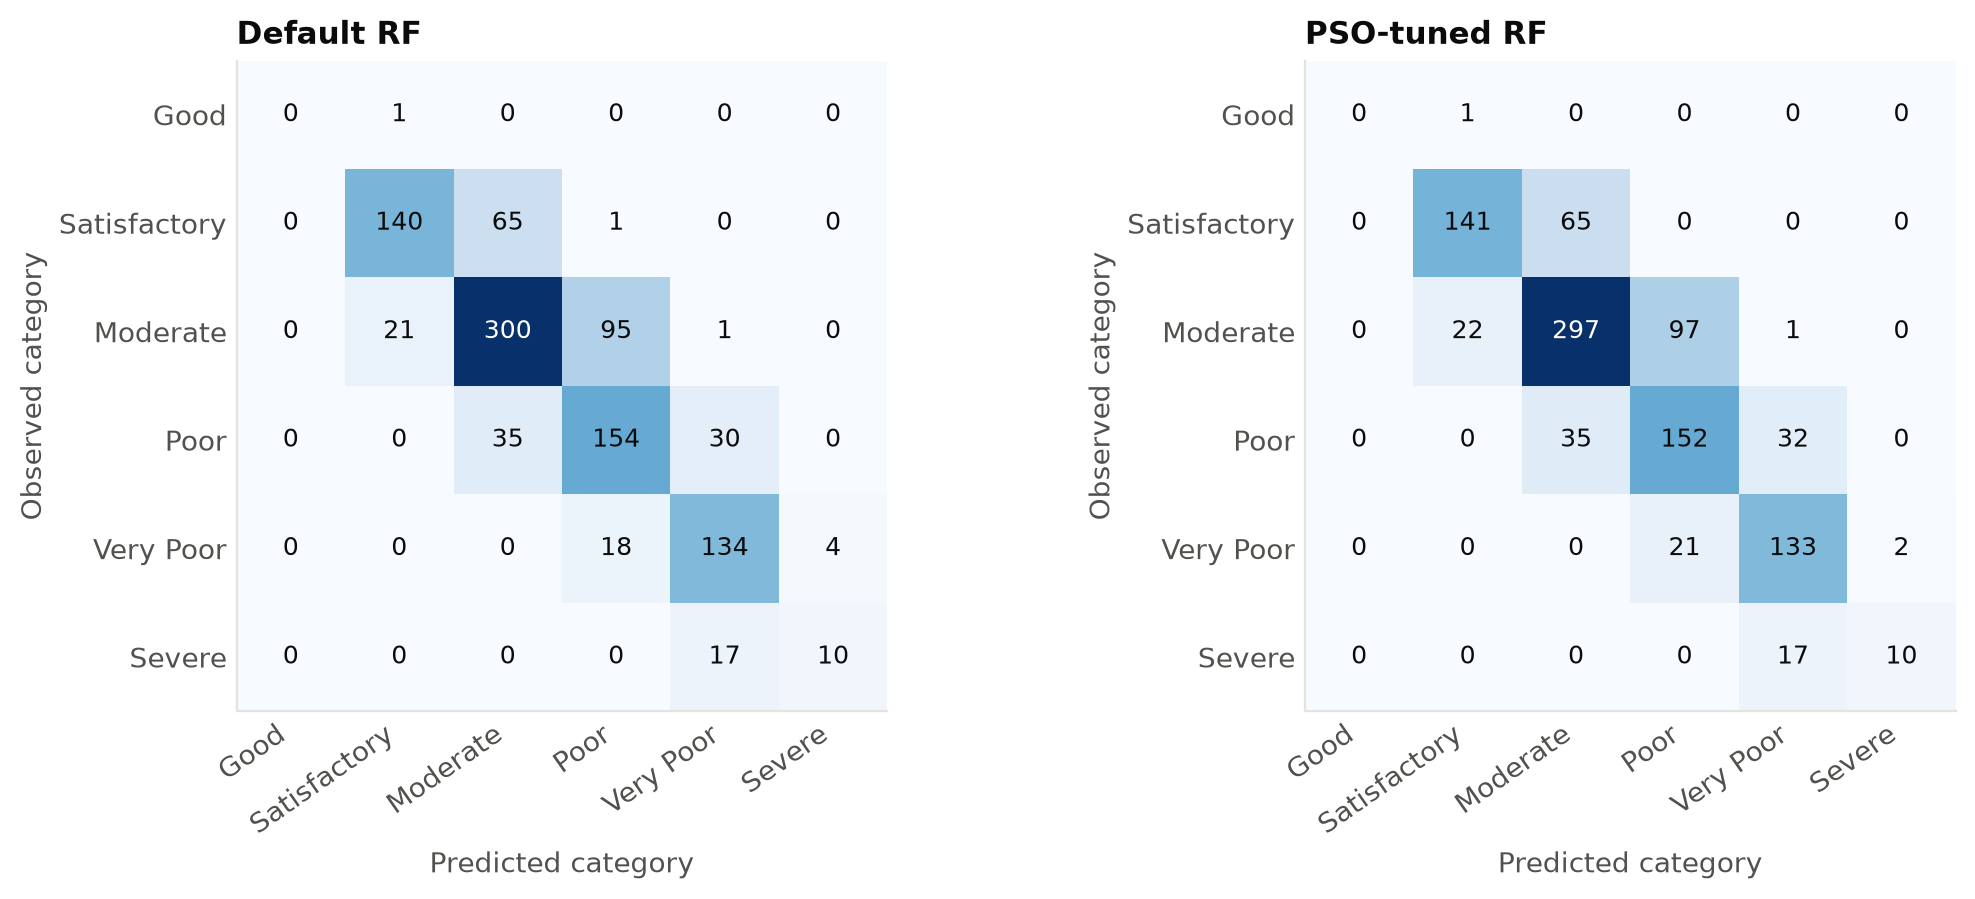
\includegraphics[width=\textwidth]{figures/14_confusion_matrices.png}
\caption{CPCB category confusion matrices on the test period}
\end{figure}

\subsection{Computational Performance}

\topic{Training Efficiency}
\begin{table}[H]
\centering
\small\setlength{\tabcolsep}{4pt}
\caption{Computational resource usage (per run)}
\begin{tabular}{|l|c|c|c|c|}
\hline
\textbf{Metric} & \textbf{PSO joint} & \textbf{RS joint} & \textbf{PSO hyp.} & \textbf{RS hyp.} \\ \hline
Fitness evaluations & 312 & 312 & 312 & 312 \\
Unique configurations trained & 312 & 312 & 307--312 & 312 \\
Forests trained per evaluation & 5 & 5 & 5 & 5 \\
Time per run (min) & 14.2--24.8 & 11.8--12.4 & 24.3--46.6 & 20.7--22.7 \\
Mean time per run (min) & 19.5 & 12.1 & 35.2 & 21.8 \\ \hline
\end{tabular}
\end{table}
The joint search is faster than the hyperparameter-only search, because each forest trains on fewer features. PSO runs take longer than random search because the swarm moves towards larger forests, which are slower to train. The search is embarrassingly parallel across runs.

\subsection{Robustness Analysis}

\topic{Stability Across Runs}
Five independent joint PSO runs with different random seeds:

\begin{table}[H]
\centering
\small
\caption{Stability across independent joint PSO runs}
\begin{tabular}{|c|c|c|c|c|c|}
\hline
\textbf{Run (seed)} & \textbf{Val. RMSE} & \textbf{Test RMSE} & \textbf{Test $R^2$} & \textbf{Features} & \textbf{Trees / depth / leaf} \\ \hline
0 (selected) & \textbf{39.73} & 33.68 & 0.882 & 14 & 224 / 18 / 2 \\
1 & 40.42 & 33.11 & 0.886 & 17 & 99 / 16 / 5 \\
2 & 39.97 & 33.53 & 0.884 & 12 & 266 / 18 / 5 \\
3 & 39.79 & 33.57 & 0.883 & 18 & 293 / 15 / 3 \\
4 & 39.81 & 33.47 & 0.884 & 18 & 187 / 22 / 3 \\ \hline
\textbf{Mean} & \textbf{39.94} & \textbf{33.47} & \textbf{0.884} & 16 & \\
\textbf{Std Dev} & \textbf{0.28} & \textbf{0.22} & \textbf{0.002} & & \\ \hline
\end{tabular}
\end{table}
Test RMSE is averaged over 10 forest seeds (the default forest averaged 33.81, SD 0.15, over the same seeds). Every joint PSO run beat the default forest on both validation and test error. However, the ranking by validation error does not carry over to the test period: the selected run (best validation) is the worst of the five on test, and run 1 (worst validation) is the best on test.

\topic{Validation Overfitting in the Larger Search}
This is the most important finding of the extension. With 38 dimensions and 312 evaluations, PSO can find feature subsets that fit the particular validation folds of 2015 to 2023 very well. Part of the 0.93-point validation gain from feature selection is therefore specific to those folds and does not transfer to 2024 to 2026. The hyperparameter-only search, with only 6 dimensions, has less freedom to overfit its validation folds: the standard deviation of its five test RMSEs is only 0.04 points, against 0.22 for the joint search. Remedies include a longer or more recent validation window, penalizing the number of features in the fitness, or averaging the forests found by several runs.

\topic{Learning Curves}
With a fixed validation window (the last 20\% of the training period), the gap between training and validation RMSE at full size is 21.1 points for the default forest (15.1 vs 36.2), 11.2 points for the hyperparameter-only PSO forest (24.8 vs 36.0) and 9.2 points for the final model (27.3 vs 36.5). PSO's regularization more than halved the overfitting gap of individual trees.

\begin{figure}[H]
\centering
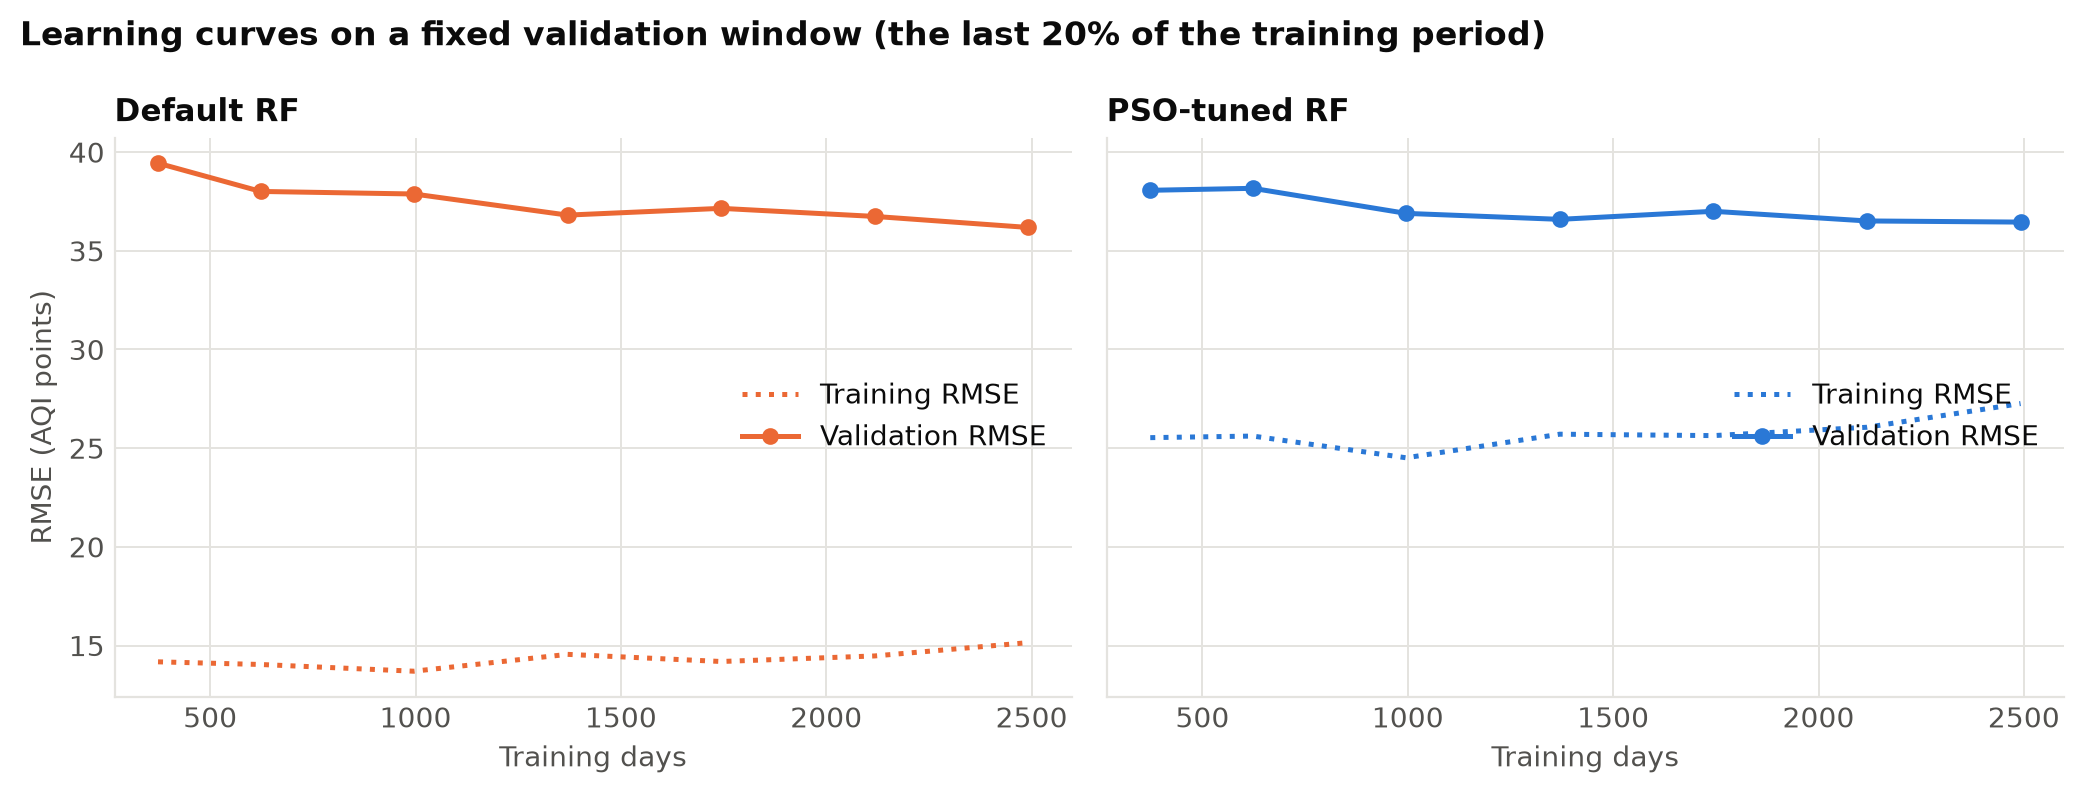
\includegraphics[width=\textwidth]{figures/12_learning_curves.png}
\caption{Learning curves of the default and final PSO Random Forest}
\end{figure}

\subsection{Discussion}

\topic{Why PSO Works Here}
Several factors contribute:
\begin{enumerate}
\item \textbf{Guided search:} Sharing the global best moves particles quickly to good regions, which is why PSO beat random search in both search spaces, and by more in the larger one
\item \textbf{No gradient dependence:} The noisy, stepped validation error and the binary feature switches are handled naturally
\item \textbf{Exploration then exploitation:} Decreasing inertia gave a broad early search and a focused late search, visible in the diversity curve
\item \textbf{Physically sensible selection:} PSO kept wind, rain and radiation and discarded redundant humidity, pressure and lag features without being told which variables matter
\end{enumerate}

\topic{Why the Test Gain over the Default Is Small}
\begin{itemize}
\item Random Forest defaults are already strong on tabular data, so there is little error left for tuning to remove
\item AQI history carries most of the predictive signal (88\% of total importance), and every model uses it
\item The largest gain came from features and model choice: moving from persistence to any learned model cut RMSE by 6 to 7 points; tuning changed it by 0.1 to 0.3
\item In the joint search, part of the validation gain was overfitting to the validation folds
\end{itemize}

\topic{Limitations}
\begin{itemize}
\item \textbf{Not statistically significant:} Neither PSO model is significantly better than the default forest on the test period
\item \textbf{Validation overfitting:} The selected joint model was 2.3\% better on validation than the hyperparameter-only model but 0.6\% worse on test
\item \textbf{Linear models competitive:} Ridge regression matched the forests, so the forest's complexity is not essential here
\item \textbf{Reactive forecasts:} Sharp jumps are followed a day late
\item \textbf{Observed, not forecast, weather:} The model uses today's weather; tomorrow's forecast weather could add information but is not in the archive used
\item \textbf{Single city:} Results apply to Delhi
\end{itemize}

\topic{Practical Implications}
\begin{itemize}
\item The model forecasts next-day AQI within about 25 AQI points on average, and flags \emph{Very Poor} days with AUC 0.986
\item It needs only 14 inputs instead of 32, which simplifies data collection for deployment
\item Retraining each year is advisable, given the downward trend in Delhi's AQI
\end{itemize}

\begin{figure}[H]
\centering
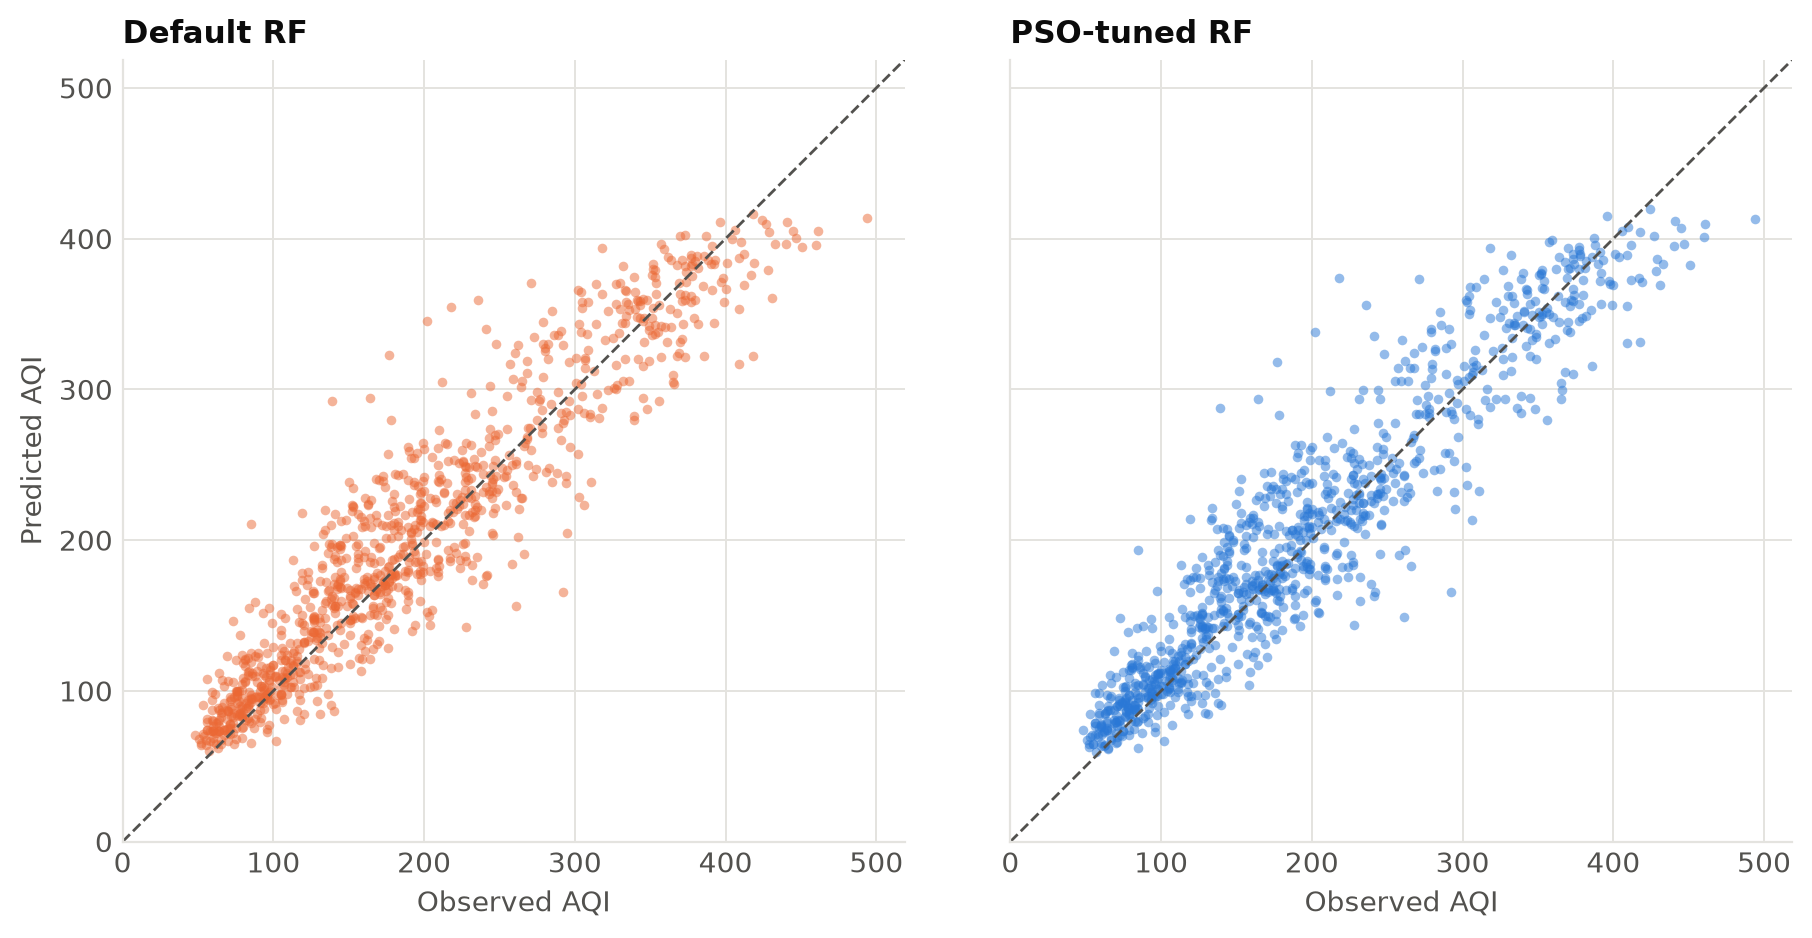
\includegraphics[width=\textwidth]{figures/10_actual_vs_predicted.png}
\caption{Model performance before optimization (left, default RF) and after PSO optimization (right)}
\end{figure}

%================================================================ 0.8
\section{Conclusion}
This project built and evaluated a Random Forest optimized by Particle Swarm Optimization for next-day AQI forecasting in Delhi, using 4,170 days of official CPCB bulletins and ERA5 weather from 2015 to 2026. PSO was implemented from first principles and verified on benchmark functions, where it solved the Sphere function to machine precision.

PSO searched the six Random Forest hyperparameters and the choice of input features together, in a 38-dimensional space with threshold-based feature switches. It reduced walk-forward validation RMSE by 4.3\% (41.52 to 39.73), twice the 2.1\% reached by tuning hyperparameters alone, and it beat random search with the same budget in both search spaces, by a wider margin in the larger one. It kept 14 of 32 features, consistently choosing wind, rain and radiation and discarding redundant humidity, pressure and lag variables.

On the held-out 2024--2026 period, the selected model achieved an RMSE of 33.77 and an $R^2$ of 0.882, 16.0\% better than persistence. Averaged over its five runs, joint PSO gave the lowest test RMSE of any search (33.47, 1.0\% below the default forest). However, the selected model's gain over the default forest was small (0.25\%) and not statistically significant, and it was slightly worse than the hyperparameter-only model, showing that the larger search partly overfitted its validation folds. PSO is an effective optimizer for this task, but for next-day AQI forecasting, good features and weather inputs matter more than tuning, and a larger search space must be paired with a more robust validation scheme.

%================================================================ 0.9
\section{Future Work}
While this project establishes a solid foundation, several directions remain for future investigation:

\subsection{Methodological Enhancements}

\topic{Better Inputs}
\textbf{Forecast Weather:} Use tomorrow's numerical weather forecast instead of today's observed weather, so the model can anticipate changes in wind and rain rather than react to them.

\textbf{Fire and Emission Data:} Add satellite fire counts from Punjab and Haryana and festival calendars, which drive the sharp autumn jumps the model currently misses.

\textbf{Multi-City Data:} Train one model across several Indo-Gangetic cities to learn shared regional patterns.

\topic{Improved Optimization Strategies}
\textbf{More Robust Fitness:} Penalize the number of features, use a more recent validation window, or evaluate each particle on several forest seeds, so the joint search overfits its validation folds less.

\textbf{Ensembles of Runs:} Average the forests found by several PSO runs; the five-run mean test RMSE (33.47) suggests this would be more reliable than picking one run.

\textbf{Other Nature-Inspired Optimizers:} Compare PSO with Genetic Algorithms, Differential Evolution and Grey Wolf Optimizer on the same budget and fitness function.

\textbf{Weighted Fitness:} Optimize an error that weights \emph{Very Poor} and \emph{Severe} days more heavily, since those forecasts matter most for public health.

\textbf{Surrogate-Assisted PSO:} Use a cheap surrogate model of the fitness to reduce the cost of each search.

\topic{Model Extensions}
\textbf{Gradient Boosting and Deep Models:} Apply the same PSO framework to gradient boosting and to sequence models such as LSTMs, which have more hyperparameters and may gain more from tuning.

\textbf{Probabilistic Forecasts:} Provide prediction intervals, so that alerts can be issued with a stated level of confidence.
